% !TEX root = main.tex
% !TEX options = -shell-escape
\documentclass[10pt]{article}
\usepackage{preamble}

\title{Homological Algebra and Embedding Theory\\in the Structured Knowledge Management Problem\\[6pt]\large DRAFT}
\author{
  Xinze Li\thanks{Department of Mathematics, University of Toronto}
}
\date{\today}

\begin{document}

\maketitle

\begin{abstract}
Every piece of structured knowledge is a finite string over a finite alphabet. We define the \emph{astrolabe file}: a finite subset $\mathbb{A} \subset H^+ \times H \times R$ of semantic simplices whose reference fields are unconstrained. The \emph{multiplicity profile} $\boldsymbol{\mu}(\sigma)$ records how many times each vertex appears in a reference list, decomposing each stage layer into its finest combinatorial partition. Grouping restriction maps by vertex yields $N$ boundary operators $\partial^{(1)}, \ldots, \partial^{(N)}$ that pairwise anticommute (\emph{multicomplex theorem}), making each stage layer a $\mathbb{Z}^N$-graded multicomplex. The classical identity $\partial^2 = 0$ is a single linear combination of the $\binom{N+1}{2}$ anticommutativity equations; homology, long exact sequences, and the snake lemma follow as corollaries.

Adding the classical constraint (all references point to vertices) recovers the geometric interpretations of algebraic topology. Adding LLM embeddings gives a \emph{stage embedding tower} $W_{m+1} = \bigwedge W_m$ with exterior algebra geometry; topology and geometry coexist, and their inconsistency pinpoints structural gaps. We prove an \emph{embedding obstruction theorem}: the topological complexity of a knowledge base gives a lower bound on embedding dimension, and give formal characterizations of hallucination, scaling saturation, ``understanding vs.\ memorization,'' and chain-of-thought reasoning.

Merging knowledge bases is not a special operation: disjoint union followed by cross-references, with homological invariants tracking the structural effect. The algebraic core is mechanically verified in Lean~4 (zero \texttt{sorry}). The data format \texttt{astrolabe.json} and a reference implementation are open-source.
\end{abstract}

\tableofcontents
\newpage 
\section{Introduction}
\label{sec:introduction}

The dominant format for communicating structured knowledge remains the PDF document~\cite{Lamport1994}. A \LaTeX\ file is a linear stream of characters whose logical structure (sections, theorems, proofs, cross-references) exists only as typesetting conventions. The dependency between Theorem~3.2 and Definition~2.1 has no machine-readable representation; it must be reconstructed by the reader from context.

\begin{figure}[h]
\centering
\begin{tikzpicture}[
  code/.style={draw, rounded corners=2pt, fill=gray!5, font=\ttfamily\scriptsize, text=black, inner sep=4pt, align=left},
  hl/.style={text=red!70!black, font=\ttfamily\scriptsize\bfseries},
  arr/.style={->, >=Stealth, thin, red!60!black}
]
% Definition block
\node[code] (def) at (0,0) {
  \textbackslash begin\{definition\}\textcolor{red!70!black}{\textbackslash label\{def:compact\}}\\
  A subset $K \subseteq \mathbb{R}^n$ is compact if\\
  every open cover has a finite subcover.\\
  \textbackslash end\{definition\}
};
% Prose block
\node[code] (thm) at (7.5,0) {
  Every bounded sequence in $\mathbb{R}^n$\\
  has a convergent subsequence\\
  (by \textcolor{red!70!black}{\textbackslash ref\{def:compact\}}).
};
% Arrow
\draw[arr] ([xshift=-2pt]thm.west) -- ([xshift=2pt]def.east);
\end{tikzpicture}
\caption{A \LaTeX\ cross-reference: \texttt{\textcolor{red!70!black}{\textbackslash label}} and \texttt{\textcolor{red!70!black}{\textbackslash ref}} create a string-level link between two locations. The reference records \emph{that} Theorem~3.2 cites Definition~2.1 but not \emph{why}; the nature of the dependency (used as a hypothesis? as a special case?) must be inferred from surrounding prose.}
\label{fig:latex-ref}
\end{figure}

This is, in a precise sense, the weakest possible structure: a flat string with no first-class morphisms.

Personal knowledge management tools such as Roam Research~\cite{RoamResearch}, Obsidian~\cite{Obsidian}, Logseq~\cite{Logseq}, and Tana~\cite{Tana} introduced bidirectional links, turning notes into graphs. These links, however, lack type information, directional semantics, and composability.

\begin{figure}[h]
\centering
\begin{tikzpicture}[
  note/.style={draw, rounded corners=2pt, fill=gray!5, font=\small, inner sep=4pt, align=left, text width=3.2cm},
  link/.style={->, >=Stealth, thin, gray}
]
\node[note] (ml) at (0,0) {\textbf{Machine Learning}\\[2pt]{\scriptsize A field of AI that uses\\statistical methods to...\\[2pt]\texttt{[[Neural Networks]]}\\[1pt]\texttt{[[Deep Learning]]}\\$\vdots$}};
\node[note] (nn) at (5.5,1.2) {\textbf{Neural Networks}\\[2pt]{\scriptsize Computational models\\inspired by biological...\\[2pt]\texttt{[[Deep Learning]]}\\$\vdots$}};
\node[note] (dl) at (5.5,-1.2) {\textbf{Deep Learning}\\[2pt]{\scriptsize A subset of ML using\\multi-layer networks...\\[2pt]\texttt{[[Machine Learning]]}\\$\vdots$}};
\draw[link] (ml) -- (nn);
\draw[link] (ml) -- (dl);
\draw[link] (nn) -- (dl);
\draw[link, bend left=40] (dl) to (ml);
\end{tikzpicture}
\caption{Obsidian/Logseq: each node is a note file containing prose and \texttt{[[wikilinks]]}. Links are directed (from the note containing the link to the target) but carry no information about the nature of the relationship.}
\label{fig:pkm-links}
\end{figure}

Knowledge graphs in the RDF/OWL tradition~\cite{Bordes2013} address this limitation by introducing typed edges. However, the type system is a fixed enumeration: adding a new relationship type requires modifying the schema itself.

\begin{figure}[h]
\centering
\begin{tikzpicture}[
  dot/.style={circle, fill, inner sep=1.5pt},
  typed/.style={->, >=Stealth, thin}
]
\node[dot] (ml) at (0,0) {};
\node[dot] (nn) at (5,0) {};
\node[dot] (dl) at (2.5,1.3) {};
\node[font=\small, anchor=north] at (ml.south) {Machine Learning};
\node[font=\small, anchor=north] at (nn.south) {Neural Networks};
\node[font=\small, anchor=south] at (dl.north) {Deep Learning};
\draw[typed] (ml) -- node[below, font=\scriptsize\ttfamily] {hasTopic} (nn);
\draw[typed] (ml) -- node[left, font=\scriptsize\ttfamily] {includes} (dl);
\draw[typed] (dl) -- node[right, font=\scriptsize\ttfamily] {isA} (nn);
\end{tikzpicture}
\caption{RDF-style knowledge graph: edges carry a type from a fixed enumeration (\texttt{implies}, \texttt{uses}, \texttt{subsetOf}, \ldots). The type vocabulary is closed; extending it requires schema modification.}
\label{fig:rdf-kg}
\end{figure}

Spivak and Kent~\cite{Spivak2012} proposed \emph{ologs} (ontology logs) as a categorical framework for knowledge representation: objects are types, morphisms are functional relations, and the category-theoretic structure enforces consistency.

\begin{figure}[h]
\centering
\begin{tikzcd}[column sep=large, row sep=large]
\text{a bounded sequence} \arrow[r, "\text{has}"] \arrow[d, "\text{is}"'] & \text{a convergent subsequence} \arrow[d, "\text{is}"] \\
\text{a sequence in } \mathbb{R}^n \arrow[r, "\text{lives in}"'] & \text{a subset of } \mathbb{R}^n
\end{tikzcd}
\caption{An olog~\cite{Spivak2012}: objects are types, morphisms are functional relations, and the diagram commutes. Morphisms are restricted to functions and cannot carry open-ended content.}
\label{fig:olog}
\end{figure}

This was a significant conceptual advance. However, ologs restrict morphisms to functional relations (every object maps to exactly one target) and do not provide a foundation from finite strings, a semantic metric, or an embedding theory. Moreover, the framework has seen limited software adoption in the years since its introduction.

\subsection{Motivation: The Autoformalization Gap}

Our work originates from a concrete software design problem in the formalization of mathematics. In Lean~4~\cite{mathlib4}, the \texttt{leanblueprint} tool~\cite{Massot2020} provides a visual map from informal mathematical statements to their formal counterparts. Dependencies are declared via \LaTeX\ macros: \verb|\uses{lem:foo}| declares that the current statement depends on \texttt{lem:foo}, and \verb|\lean{Bar.baz}| links it to the Lean declaration \texttt{Bar.baz}. These macros generate a dependency graph (Figure~\ref{fig:blueprint-vs-decl}, left), but each edge carries only the label ``uses'' with no further semantic content. LeanArchitect~\cite{Zhu2026} automates blueprint generation, yet the fundamental gap remains: the \emph{meaning} of each dependency is not represented.

\begin{figure}[ht]
\centering
\begin{tikzpicture}[
  bp/.style={draw, rounded corners=2pt, fill=green!10, font=\scriptsize, inner sep=3pt, minimum width=1.4cm, minimum height=0.5cm},
  decl/.style={circle, fill, inner sep=1.5pt},
  arr/.style={->, >=Stealth, thin},
  darr/.style={->, >=Stealth, thin, red!60!black}
]
% Left: Blueprint graph (manual, via \uses{} macro)
\node[font=\small\bfseries] at (1.5, 2.8) {Blueprint};
\node[bp] (la) at (1.5, 2) {\texttt{length\_append}};
\node[bp] (lm) at (0, 0.5) {\texttt{length\_map}};
\node[bp] (mm) at (3, 0.5) {\texttt{map\_map}};
\node[bp] (len) at (1.5, -0.8) {\texttt{List.length}};
\draw[arr] (la) -- node[left, font=\tiny] {uses} (lm);
\draw[arr] (la) -- node[right, font=\tiny] {uses} (len);
\draw[arr] (lm) -- node[left, font=\tiny] {uses} (len);
\draw[arr] (mm) -- node[right, font=\tiny] {uses} (len);

% Right: Declaration-level graph (compiler-extracted, finer-grained)
\node[font=\small\bfseries] at (7.5, 2.8) {Declaration graph};
\node[decl, label={[font=\scriptsize]above:\texttt{length\_append}}] (a) at (7.5, 2) {};
\node[decl, label={[font=\scriptsize]left:\texttt{length\_map}}] (b) at (5.8, 0.8) {};
\node[decl, label={[font=\scriptsize]right:\texttt{map\_map}}] (c) at (9.2, 0.8) {};
\node[decl, label={[font=\scriptsize]below:\texttt{List.length}}] (d) at (7.5, -0.3) {};
\node[decl, label={[font=\scriptsize]left:\texttt{List.rec}}] (rec) at (5.5, -0.5) {};
\node[decl, label={[font=\scriptsize]right:\texttt{Nat.add}}] (add) at (9.5, -0.5) {};
\node[decl, label={[font=\scriptsize]below:\texttt{List.map}}] (map) at (7.5, -1.3) {};
\draw[darr] (a) -- (b);
\draw[darr] (a) -- (d);
\draw[darr] (a) -- (add);
\draw[darr] (b) -- (d);
\draw[darr] (b) -- (map);
\draw[darr] (c) -- (map);
\draw[darr] (c) -- (rec);
\draw[darr] (d) -- (rec);
\draw[darr, dashed, gray] (a) to[bend right=15] (rec);
\draw[darr, dashed, gray] (a) to[bend left=15] (map);
\end{tikzpicture}
\caption{Left: a \texttt{leanblueprint} dependency graph for basic list lemmas. Each edge is labeled ``uses'' via \texttt{\textbackslash uses\{\}} macros. Right: the declaration-level dependency graph extracted from Lean~4 compilation artifacts~\cite{LiPengSeverini2026}. The compiler graph reveals additional nodes (\texttt{List.rec}, \texttt{Nat.add}, \texttt{List.map}) and implicit dependencies (dashed). Both representations lose the semantic content of each edge.}
\label{fig:blueprint-vs-decl}
\end{figure}

Autoformalization~\cite{Wu2022, Jiang2023} aims to translate informal mathematics directly into formal proofs. The gap between ``Draft, Sketch, and Prove'' and full autoformalization is precisely a gap in structured knowledge representation: the system needs to know not just \emph{that} \texttt{length\_append} depends on \texttt{List.length}, but \emph{how}. Does it unfold the definition? Apply it to a subterm? Use it via a rewrite? This information is present in the Lean proof term but lost in both the blueprint and the declaration graph.

In designing Astrolabe to bridge this gap, we realized that the problem is not specific to mathematics. Our prior work on the network structure of Mathlib~\cite{LiPengSeverini2026} made visible the rich structural information latent in formalized mathematics, while our work on content-addressing~\cite{LiParisSeverini2026} demonstrated the advantages of hash-based decentralized identification. Together, these revealed that dependency graphs, even when carefully extracted from compiler artifacts, lose the semantic content of each dependency. The same limitation appears across domains of structured knowledge, including legal codes~\cite{Catala}, software architecture, and scientific literature~\cite{Garfield1955, Price1965}: \emph{morphisms lack open semantics}. Edges in a knowledge graph should carry arbitrary key-value content, just as nodes do.

Every externalized form of human knowledge, whether a \LaTeX\ file, a Lean proof, a Python module, or a legal statute, is a finite string over a finite alphabet. Different parsing procedures (a compiler, an LLM, a human reader) extract different structures from the same underlying string. This observation suggests a universal foundation: start from the free monoid $A^*$ and build upward. A record can freely reference any other record. References are not restricted to ``vertices'' or ``atoms''; an edge can reference another edge, a face can reference a complex. This unconstrained reference structure is the key departure from classical simplicial topology: we impose no constraint on what $\texttt{ref}$ points to. Moreover, a reference list may contain the same vertex multiple times: the \emph{multiplicity profile} $\boldsymbol{\mu}(\sigma)$ records the exact usage pattern and provides the finest combinatorial decomposition of each stage layer.

\subsection{Methodology and Contributions}

We build from a finite alphabet $A$ to the astrolabe file $\mathbb{A} \subset H^+ \times H \times R$ (\S\ref{sec:foundations}), develop its homological algebra via the multicomplex theorem (\S\ref{sec:topology}), add embedding geometry via the stage tower (\S\ref{sec:semantics}), and implement the framework as the open-source tool \texttt{astrolabe.json} (\S\ref{sec:implementation}).

The first contribution is the \emph{Astrolabe} itself: a finite collection $\mathbb{A} \subset H^+ \times H \times R$ of semantic simplices whose reference fields are unconstrained. Each reference list carries a \emph{multiplicity profile} $\boldsymbol{\mu}(\sigma)$ recording how many times each vertex appears. The profile decomposition is the finest partition of each stage layer; degree and stage, the two decompositions that organize classical simplicial topology, are both projections of the profile (\S\ref{sec:foundations}).

The core algebraic result is the \emph{multicomplex theorem} (\S\ref{sec:topology}): grouping restriction maps by which vertex they remove yields $N$ boundary operators $\partial^{(1)}, \ldots, \partial^{(N)}$, one per vertex, that pairwise anticommute. This is strictly stronger than $\partial^2 = 0$: the classical identity is a single linear combination of $\binom{N+1}{2}$ independent equations. Homology, cohomology, long exact sequences, and the snake lemma all follow as corollaries of the anticommutativity, and hold unconditionally.

On the geometric side, LLM embeddings on vertices extend to every stage via a recursive \emph{stage embedding tower} $W_{m+1} = \bigwedge W_m$ (\S\ref{sec:semantics}). The tower is forced, not chosen: stage decomposition requires the next ambient space to contain exterior products of all degrees, which is exactly $\bigwedge W_m$. The topological complexity $k^*$ of a knowledge base gives a provable lower bound $d \geq k^*$ on embedding dimension (the \emph{embedding obstruction theorem}). Grade mixing yields a distance decomposition with an irreducible cross-grade component that has no analogue in classical simplicial geometry.

These tools give formal characterizations of four AI frontier problems: hallucination (grade-stratified: type confusion vs.\ structural flattening), scaling saturation (per-stage: increasing $d$ has exponential payoff at higher stages), the distinction between understanding and memorization (normalized volume: zero means memorizing), and chain-of-thought reasoning (stage-crossing paths exploit dimensional surplus). The characterizations are definitions with testable predictions, not metaphors (\S\ref{sec:semantics}).

On the engineering side, merging two knowledge bases requires no special operation: disjoint union followed by cross-references, with homological invariants tracking the structural effect. Plugins are typed operations (source, endo, sink) composed via the single intermediate representation \texttt{astrolabe.json}. The unified structure reduces pipeline steps from $2p - 1$ to $p$ and annotation cost from $mn$ to $2n$ (\S\ref{sec:implementation}). The algebraic core is mechanically verified in Lean~4 with zero \texttt{sorry}; a reference implementation and the data format are open-source.

\subsection{Related Work}

\begin{itemize}
\item \textbf{Ologs}~\cite{Spivak2012}: No $A^*$ foundation, no restriction maps, no metric, no verification.
\item \textbf{AlgebraicJulia / Catlab.jl}: categorical data structures for scientific modeling. The astrolabe takes a different approach: homological invariants replace categorical universal properties as the primary structural tool.
\item \textbf{CASC}: $\texttt{ref}$ can only reference vertices; no self-enrichment.
\item \textbf{TDA for LLM} (HalluZig, TOHA, G-Detector): Empirical approaches that construct complexes from data. The Astrolabe defines complexes from knowledge structure and explains \emph{why} TDA is effective.
\item \textbf{RDF/OWL}: Edge types are fixed enumerations; no open-ended $\texttt{record}$.
\item \textbf{Obsidian / Logseq}: Edges have no semantics.
\item \textbf{leanblueprint}: Static, manual correspondence between blueprint and formalization.
\item \textbf{$\infty$-categories} (Lurie): Pure theory; no data structure, no implementation.
\end{itemize}

\section{Foundations}
\label{sec:foundations}

We build the theory from a single starting point: a finite alphabet. Every externalized piece of knowledge is a finite string; structured knowledge is a finite sequence of key-value pairs of strings. From this minimal assumption we construct hash identifiers and a reference structure, arriving at the \emph{signature} $\Sigma = (S, h_{\mathrm{id}})$. Records in a signature are graded by the number of other records they reference, yielding a \emph{semantic simplicial complex} $\Delta(\Sigma) = \bigsqcup_{k \geq 0} \Delta_k$, on which the algebraic topology of \S\ref{sec:topology} operates. The geometric structure (semantic embeddings, metrics) is introduced in \S\ref{sec:semantics}.

\subsection{Alphabet and String Space}

\begin{definition}[Alphabet]
\label{def:alphabet}
An \emph{alphabet} is a finite set $A$. We impose no structure on $A$ beyond finiteness; it may be the set of Unicode code points, ASCII characters, or any other finite encoding.
\end{definition}

\begin{definition}[Monoid]
\label{def:monoid}
A \emph{monoid} is a triple $(M, \cdot, e)$ where $M$ is a set, $\cdot : M \times M \to M$ is an associative binary operation, and $e \in M$ is an identity element: $e \cdot m = m \cdot e = m$ for all $m \in M$.
\end{definition}

\begin{definition}[String space]
\label{def:string-space}
The \emph{string space} $A^*$ is the free monoid on $A$: the set of all finite sequences of elements of $A$, with concatenation as the monoid operation and the empty sequence $\varepsilon$ as identity.
\end{definition}

Every \LaTeX\ file, every Lean source, every JSON document, and every natural-language paragraph is an element of $A^*$ for an appropriate choice of $A$ (e.g., $A_{\mathrm{ASCII}}$ with $|A| = 128$, or the full Unicode code point set).

\begin{theorem}[Universal property of $A^*$]
\label{thm:free-monoid}
For any monoid $(M, \cdot, e)$ and any function $f : A \to M$, there exists a unique monoid homomorphism $\bar{f} : A^* \to M$ extending $f$.
\end{theorem}

In Lean~4, $A^*$ is \texttt{FreeMonoid} in Mathlib, and the universal property is \texttt{FreeMonoid.lift}, a corollary of the adjunction $\mathrm{Free} \dashv U$ between the free monoid functor and the forgetful functor. The universal property guarantees that any structure-preserving interpretation of the alphabet extends uniquely to all strings; this is the algebraic foundation of parsing.

\subsection{Record, Parsing, and Signature}

\begin{definition}[Record space]
\label{def:record-space}
A \emph{record} is a finite sequence of key-value pairs, where both keys and values are strings:
\[
  R = (A^* \times A^*)^*.
\]
A record $r = ((k_1, v_1), \ldots, (k_n, v_n)) \in R$ assigns to each key $k_i$ a value $v_i$. Keys may repeat; the order of pairs is significant.
\end{definition}

\begin{definition}[Parsing]
\label{def:parsing}
Let $\mathcal{P}_{\mathrm{fin}}(R)$ denote the set of finite subsets of $R$:
\[
\mathcal{P}_{\mathrm{fin}}(R) = \{ S \subseteq R \mid |S| < \infty \}.
\]
A \emph{parsing procedure} is a function $P : A^* \to \mathcal{P}_{\mathrm{fin}}(R)$ that maps a string to a finite set of records. Different parsing procedures extract different structures from the same string; we distinguish them by subscripts ($P_{\mathrm{compiler}}$, $P_{\mathrm{LLM}}$, etc.).
\end{definition}

\begin{example}
Consider the Lean source file $s \in A^*$:
\begin{minted}[fontsize=\scriptsize]{lean4}
theorem length_append (l1 l2 : List a) :
    (l1 ++ l2).length = l1.length + l2.length := by
  induction l1 <;> simp [*]
\end{minted}
\noindent Three parsers extract different sets of records from the same string:
\begin{itemize}
\item $P_{\mathrm{compiler}}(s)$: the Lean~4 compiler reads \texttt{.ilean} artifacts and produces one record per declaration. Writing each record as an element of $R = (A^* \times A^*)^*$:
\begin{align*}
r_1 &= ((\texttt{name},\; \texttt{length\_append}),\; (\texttt{sort},\; \texttt{theorem}),\; (\texttt{stmt},\; \ldots\,)) \in R, \\
r_2 &= ((\texttt{name},\; \texttt{List.length}),\; (\texttt{sort},\; \texttt{definition})) \in R, \\
r_3 &= ((\texttt{name},\; \texttt{List.append}),\; (\texttt{sort},\; \texttt{definition})) \in R, \\
r_4 &= ((\texttt{name},\; \texttt{Nat.add}),\; (\texttt{sort},\; \texttt{definition})) \in R.
\end{align*}
Thus $P_{\mathrm{compiler}}(s) = \{r_1, r_2, r_3, r_4\} \in \mathcal{P}_{\mathrm{fin}}(R)$.

\item $P_{\mathrm{LLM}}(s)$: a language model reads the same file as natural language and extracts records for each mathematical concept:
\[
P_{\mathrm{LLM}}(s) = \bigl\{\,
((\texttt{name},\; \texttt{list concatenation}),\; (\texttt{sort},\; \texttt{concept})),\;\ldots
\,\bigr\} \in \mathcal{P}_{\mathrm{fin}}(R).
\]

\item $P_{\mathrm{AST}}(s)$: a syntax-level parser extracts the abstract syntax tree, producing records for each node:
\[
P_{\mathrm{AST}}(s) = \bigl\{\,
((\texttt{name},\; \texttt{length\_append}),\; (\texttt{sort},\; \texttt{theorem})),\;\ldots
\,\bigr\} \in \mathcal{P}_{\mathrm{fin}}(R).
\]
\end{itemize}
\noindent In general $P_{\mathrm{compiler}}(s) \neq P_{\mathrm{LLM}}(s) \neq P_{\mathrm{AST}}(s)$: different parsers extract different records from the same string. The framework is indifferent to domain; the same construction applies to Python modules, legal statutes, or biological databases.
\end{example}

\begin{definition}[Identity hash]
\label{def:identity-hash}
An \emph{identity hash} is a function $h_{\mathrm{id}} : H^* \times R \to H$ that maps a vertex list and a record to an identifier in $H$ (in practice, $H = \{0,\ldots,9,\texttt{a},\ldots,\texttt{f}\}^{12}$, the set of 12-character hexadecimal strings). The hash is computed from the concatenation of the serialized vertex list $\texttt{ref}$ and the essential part of $\texttt{record}$:
\[
h_{\mathrm{id}}(\texttt{ref},\; \texttt{record}) = \texttt{SHA256}\bigl(\texttt{serialize}(\texttt{ref}) \;\|\; \texttt{serialize}(\texttt{record}_{\mathrm{ess}})\bigr)[:12].
\]
Two simplices are considered identical if and only if they have the same vertex list and the same essential content.
\end{definition}

The identity hash is a content-addressing mechanism~\cite{Benet2014}: a simplex's identity is determined by \emph{what it connects} ($\texttt{ref}$) and \emph{what it says} ($\texttt{record}$), not by its location. This is the same principle underlying Git commits and IPFS~\cite{Benet2014}.

\begin{example}
For a 0-simplex (vertex):
\begin{minted}[fontsize=\scriptsize]{python}
ref    = '["a1b2c3"]'
record = '{"name":"Nat.add_comm","sort":"theorem","stmt":"..."}'
h_id   = sha256(ref + record).hexdigest()[:12]  # "a1b2c3"
\end{minted}
\noindent The 0-simplex's $\texttt{ref}$ contains its own hash, so the definition is self-referential: $h_{\mathrm{id}}$ is the unique fixed point of $h \mapsto \texttt{SHA256}([h] \| \texttt{record})[:12]$.

For a 1-simplex (edge) connecting two vertices:
\begin{minted}[fontsize=\scriptsize]{python}
ref    = '["a1b2c3","b2c3d4"]'
record = '{"sort":"uses","weight":"0.9"}'
h_id   = sha256(ref + record).hexdigest()[:12]  # "x7y8z9"
\end{minted}
\noindent The same two vertices with different $\texttt{record}$ produce a different hash---they are distinct 1-simplices. The same $\texttt{record}$ with different vertices also produces a different hash. Collision probability is $< 2^{-48}$ per pair, negligible for knowledge bases with $n < 10^6$ simplices.
\end{example}


\begin{definition}[Signature]
\label{def:signature}
A \emph{signature} is a pair $\Sigma = (S, h_{\mathrm{id}})$ where $S$ is a finite set of records and $h_{\mathrm{id}} : S \hookrightarrow H$ is an injective identity hash. Since $h_{\mathrm{id}}$ is injective, it induces a dictionary structure: each record $r \in S$ is uniquely indexed by its hash $h_{\mathrm{id}}(r)$.
\end{definition}

\subsection{Semantic Simplicial Complex}

\begin{definition}[Semantic simplex]
\label{def:semantic-simplex}
Let $\Sigma = (S, h_{\mathrm{id}})$ be a signature. A \emph{semantic simplex} is a triple $(\texttt{hash},\; \texttt{ref},\; \texttt{record})$ where:
\begin{itemize}
\item $\texttt{hash} \in H$ is the identity hash, generated by $h_{\mathrm{id}}$ from $\texttt{ref}$ and the essential part of $\texttt{record}$.
\item $\texttt{ref} = [v_0, v_1, \ldots, v_k]$ is an ordered list of hashes in $H$, called the \emph{vertex list}.
\item $\texttt{record} \in (A^* \times A^*)^*$ is the \emph{semantic content}: an open collection of key-value pairs.
\end{itemize}
The \emph{dimension} of the simplex is
\[
\dim(\sigma) = |\texttt{ref}| - 1.
\]
A 0-simplex (vertex) has $\texttt{ref} = [v_0]$ where $v_0$ is its own hash---it is its own sole vertex. A $k$-simplex ($k \geq 1$) has $\texttt{ref} = [v_0, \ldots, v_k]$ referencing $k + 1$ vertices. The ordering of $\texttt{ref}$ determines the face maps and the signs in $\partial$.

We write $\Delta_k = \{ \sigma \in S \mid |\texttt{ref}(\sigma)| = k + 1 \}$ for the set of all $k$-semantic simplices.
\end{definition}

\begin{figure}[ht]
\centering
\begin{tabular}{|l|c|c|c|}
\hline
& $k = 0$ (vertex) & $k = 1$ (edge) & $k = 2$ (face) \\
\hline
% --- Row 1: geometry ---
\textbf{Simplex}
&
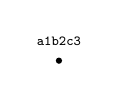
\begin{tikzpicture}[baseline=-5pt,
  v/.style={circle, fill, inner sep=0.8pt}]
\node[v] (p) at (0,0) {};
\node[font=\tiny, above=2pt] at (p) {\texttt{a1b2c3}};
\end{tikzpicture}
&
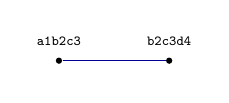
\begin{tikzpicture}[baseline=-5pt,
  v/.style={circle, fill, inner sep=0.8pt}]
\node[v] (a) at (0,0) {};
\node[v] (b) at (1.4,0) {};
\draw[very thin, blue!60!black] (a)--(b);
\node[font=\tiny, above=2pt] at (a) {\texttt{a1b2c3}};
\node[font=\tiny, above=2pt] at (b) {\texttt{b2c3d4}};
\end{tikzpicture}
&
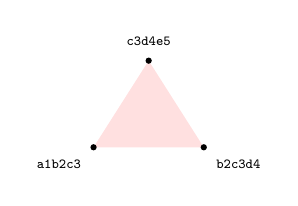
\begin{tikzpicture}[baseline=-5pt,
  v/.style={circle, fill, inner sep=0.8pt}]
\coordinate (a) at (0,0);
\coordinate (b) at (1.4,0);
\coordinate (c) at (0.7,1.1);
\fill[red!12] (a)--(b)--(c)--cycle;
\node[v] at (a) {};
\node[v] at (b) {};
\node[v] at (c) {};
\node[font=\tiny, below left=1pt] at (a) {\texttt{a1b2c3}};
\node[font=\tiny, below right=1pt] at (b) {\texttt{b2c3d4}};
\node[font=\tiny, above=2pt] at (c) {\texttt{c3d4e5}};
\end{tikzpicture}
\\
\hline
% --- Row 2: h_id ---
$h_{\mathrm{id}}$
&
\texttt{\scriptsize a1b2c3}
&
\textcolor{blue!60!black}{\texttt{\scriptsize x7y8z9}}
&
\textcolor{red!40!black}{\texttt{\scriptsize q1r2s3}}
\\
\hline
% --- Row 3: JSON ---
\texttt{ssc.json}
&
\begin{minipage}[t]{0.25\textwidth}
\begin{minted}[fontsize=\tiny,frame=none,bgcolor=gray!5]{json}
"a1b2c3": {
 "ref": ["a1b2c3"],
 "record": {
  "name": "Nat.add_comm",
  "sort": "theorem",
  "stmt": "..."
 }
}
\end{minted}
\end{minipage}
&
\begin{minipage}[t]{0.25\textwidth}
\begin{minted}[fontsize=\tiny,frame=none,bgcolor=gray!5]{json}
"x7y8z9": {
 "ref": ["a1b2c3",
         "b2c3d4"],
 "record": {
  "sort": "uses",
  "weight": "0.9"
 }
}
\end{minted}
\end{minipage}
&
\begin{minipage}[t]{0.25\textwidth}
\begin{minted}[fontsize=\tiny,frame=none,bgcolor=gray!5]{json}
"q1r2s3": {
 "ref": ["a1b2c3",
         "b2c3d4",
         "c3d4e5"],
 "record": {
  "sort": "joint_step",
  "method": "apply"
 }
}
\end{minted}
\end{minipage}
\\
\hline
\end{tabular}
\caption{Semantic simplices of dimension $0$, $1$, $2$. Top: geometric representation with vertex $h_{\mathrm{id}}$'s (blue). Middle: dimension and simplex $h_{\mathrm{id}}$. Bottom: \texttt{ssc.json} storage format. Each simplex is a triple $(\texttt{hash}, \texttt{ref}, \texttt{record})$; the vertex list $\texttt{ref}$ has length $k+1$.}
\label{fig:simplices}
\end{figure}

\begin{definition}[Semantic simplicial complex]
\label{def:semantic-complex}
The \emph{semantic simplicial complex} is the graded set
\[
\Delta(\Sigma) = \bigsqcup_{k \geq 0} \Delta_k
\]
where $\Delta_k = \{ \sigma \in S \mid |\texttt{ref}(\sigma)| = k + 1 \}$. The index $k$ is the dimension: $\Delta_0$ contains all vertices, $\Delta_1$ all edges, $\Delta_2$ all faces, and so on.
\end{definition}

\begin{figure}[ht]
\centering
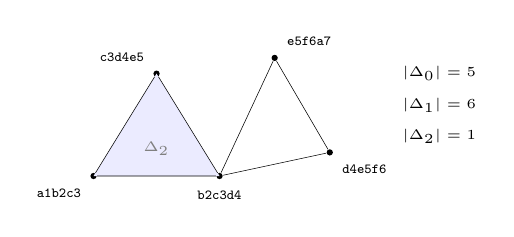
\begin{tikzpicture}[
  v/.style={circle, fill, inner sep=0.8pt},
  lbl/.style={font=\tiny}
]
\node[v] (A) at (0, 0) {};
\node[v] (B) at (1.6, 0) {};
\node[v] (C) at (0.8, 1.3) {};
\node[v] (D) at (3.0, 0.3) {};
\node[v] (E) at (2.3, 1.5) {};

\node[lbl, below left=1pt] at (A) {\texttt{a1b2c3}};
\node[lbl, below=2pt] at (B) {\texttt{b2c3d4}};
\node[lbl, above left=1pt] at (C) {\texttt{c3d4e5}};
\node[lbl, below right=1pt] at (D) {\texttt{d4e5f6}};
\node[lbl, above right=1pt] at (E) {\texttt{e5f6a7}};

\fill[blue!8] (A.center) -- (B.center) -- (C.center) -- cycle;
\draw[very thin] (A)--(B) (B)--(C) (A)--(C);
\draw[very thin] (B)--(D) (D)--(E) (B)--(E);

\node[font=\tiny, gray] at (0.8, 0.35) {$\Delta_2$};

\node[font=\tiny, anchor=west] at (3.8, 1.3) {$|\Delta_0| = 5$};
\node[font=\tiny, anchor=west] at (3.8, 0.9) {$|\Delta_1| = 6$};
\node[font=\tiny, anchor=west] at (3.8, 0.5) {$|\Delta_2| = 1$};
\end{tikzpicture}
\caption{A semantic simplicial complex $\Delta(\Sigma)$ with five vertices, six edges, and one filled face (the triangle $[v_0, v_1, v_2]$). The triangle $[v_1, v_3, v_4]$ is \emph{not} filled: the three edges exist but no 2-simplex with $\texttt{ref} = [v_1, v_3, v_4]$ is in $S$.}
\label{fig:complex}
\end{figure}

\begin{definition}[Face maps]
\label{def:face-maps}
For a $k$-simplex $\sigma$ with $\texttt{ref} = [v_0, \ldots, v_k]$, the \emph{$i$-th face map} is
\[
d_i(\sigma) = [v_0, \ldots, \hat{v}_i, \ldots, v_k], \qquad 0 \leq i \leq k,
\]
where $\hat{v}_i$ denotes omission of the $i$-th entry. The result is a vertex list of length $k$; the corresponding $(k-1)$-simplex may or may not exist in $S$.
\end{definition}

\begin{proposition}[Simplicial identity]
\label{prop:simplicial-identity}
The face maps satisfy
\[
d_i \circ d_j = d_{j-1} \circ d_i \quad \text{for } i < j.
\]
\end{proposition}

\begin{proof}
Removing $v_j$ first and then $v_i$ ($i < j$): after removing $v_j$, the index of $v_i$ is unchanged (since $i < j$), so the second removal is $d_i$. Removing $v_i$ first and then $v_j$: after removing $v_i$, the index of $v_j$ shifts down by one to $j - 1$, so the second removal is $d_{j-1}$. Both operations yield the same list with $v_i$ and $v_j$ omitted.
\end{proof}

The simplicial identity ensures that $\Delta(\Sigma)$ together with the face maps forms a \emph{semi-simplicial set}: a graded set with face maps satisfying $d_i \circ d_j = d_{j-1} \circ d_i$, but without degeneracy maps. The absence of degeneracies reflects the fact that a face $d_i(\sigma)$ may not exist as a simplex in $S$---a knowledge base may record a ternary relationship without recording all pairwise relationships.

\begin{figure}[ht]
\centering
\begin{tikzpicture}[
  v/.style={circle, fill=blue!70!black, inner sep=1.5pt},
  lbl/.style={font=\small, blue!70!black},
  arr/.style={->, >=Stealth, gray, thick}
]
\coordinate (a) at (0, 0);
\coordinate (b) at (2.2, 0);
\coordinate (c) at (1.1, 1.8);
\fill[blue!8] (a)--(b)--(c)--cycle;
\draw[semithick, blue!50!black] (a)--(b)--(c)--cycle;
\node[v] at (a) {};
\node[v] at (b) {};
\node[v] at (c) {};
\node[lbl, below left=1pt] at (a) {$v_0$};
\node[lbl, below right=1pt] at (b) {$v_1$};
\node[lbl, above=2pt] at (c) {$v_2$};
\node[font=\small] at (1.1, 0.5) {$\sigma$};
\node[font=\scriptsize, gray] at (1.1, -0.6) {$\texttt{ref} = [v_0, v_1, v_2]$};
\draw[arr] (3.0, 0.9) -- node[above, font=\small] {$d_0$} node[below, font=\scriptsize, red!60!black] {remove $v_0$} (5.0, 0.9);
\node[v] (r1) at (5.8, 0.4) {};
\node[v] (r2) at (7.3, 1.4) {};
\draw[semithick, blue!50!black] (r1)--(r2);
\node[lbl, below=2pt] at (r1) {$v_1$};
\node[lbl, above=2pt] at (r2) {$v_2$};
\node[font=\scriptsize, gray] at (6.9, -0.1) {$\texttt{ref} = [v_1, v_2]$};
\end{tikzpicture}
\caption{The face map $d_0$ applied to a 2-simplex $\sigma$: removing $v_0$ from $\texttt{ref} = [v_0, v_1, v_2]$ yields the 1-simplex $[v_1, v_2]$. Similarly, $d_1$ removes $v_1$ to give $[v_0, v_2]$, and $d_2$ removes $v_2$ to give $[v_0, v_1]$.}
\label{fig:face-maps}
\end{figure}

The face map $d_i$ answers the question: ``what remains if we forget the $i$-th vertex?'' For a 1-simplex $\sigma$ with $\texttt{ref} = [v_0, v_1]$:
\[
d_0(\sigma) = [v_1], \qquad d_1(\sigma) = [v_0].
\]
These are the two endpoints of the edge. In the free category (\S\ref{sec:category}), $d_1$ and $d_0$ recover the source and target maps: $s(\sigma) = v_0$, $t(\sigma) = v_1$.

For a 2-simplex $\sigma$ with $\texttt{ref} = [v_0, v_1, v_2]$:
\[
d_0(\sigma) = [v_1, v_2], \qquad d_1(\sigma) = [v_0, v_2], \qquad d_2(\sigma) = [v_0, v_1].
\]
These are the three edges of the triangle. The face $d_i$ is the edge \emph{opposite} to vertex $v_i$.

The simplicial identity $d_i \circ d_j = d_{j-1} \circ d_i$ ($i < j$) ensures that removing two vertices in either order gives the same result. For instance, removing $v_0$ then $v_1$ from $[v_0, v_1, v_2]$ gives $[v_2]$, and removing $v_1$ then $v_0$ also gives $[v_2]$: $d_0 \circ d_1 = d_0 \circ d_0$.



Not every position in the complex need be occupied by a substantive simplex. We explicitly record absences:

\begin{definition}[Semantic void]
\label{def:void}
A \emph{semantic void} is a simplex whose $\texttt{record}$ has a \texttt{sort} indicating absence rather than presence:
\begin{itemize}
\item $\texttt{sort} = \texttt{"independent"}$: confirmed absence of relation.
\item $\texttt{sort} = \texttt{"missing"}$: expected relation not yet recorded.
\item $\texttt{sort} = \texttt{"induced"}$: face induced by a higher simplex, semantics pending.
\item $\texttt{sort} = \texttt{"negated"}$: explicit negation of relation.
\end{itemize}
A void has its own $\texttt{hash}$ and is a full member of $\Delta(\Sigma)$. Absence is not a gap in the data structure---it is a record with semantic content.
\end{definition}

\section{Algebraic Structure}
\label{sec:topology}

\S\ref{sec:foundations} defined the combinatorial objects that populate an astrolabe file: atoms, $k$-forms, and their stage decomposition. We now introduce algebraic structure. The uniform vertex pool property (Proposition~\ref{prop:uniform-pool}) ensures that within each stage layer $\Delta^{(m)} = \mathcal{S}_{m+1} \setminus \mathcal{S}_m$, every entry draws its references from the same hash pool $\mathcal{H}_m$. This makes each layer a natural home for the classical constructions of algebraic topology: we rename $k$-forms as $k$-simplices, define restriction maps and the boundary operator, and verify $\partial^2 = 0$.

%%% §3.1 — From Forms to Simplices (pure concept, no algebra)

\subsection{From Forms to Simplices}

\begin{definition}[Stage layer and its simplices]
\label{def:stage-layer}
The \emph{stage $m$ layer} is $\Delta^{(m)} = \mathcal{S}_{m+1} \setminus \mathcal{S}_m$, with vertex set $\mathcal{H}_m$. Its \emph{$k$-simplices} are
\[
\Delta^{(m)}_k = \mathbb{A}_k \cap \Delta^{(m)},
\]
the entries of degree $k$ that belong to stage $m$. The graded decomposition is $\Delta^{(m)} = \bigsqcup_{k \geq 1} \Delta^{(m)}_k$.
\end{definition}

The passage from $k$-form (\S\ref{sec:foundations}) to $k$-simplex is a change of perspective, not of data: the same entry in \texttt{astrolabe.json} is viewed as a combinatorial object in \S\ref{sec:foundations} and as an algebraic object carrying boundary relations here.

\begin{example}[Simplices within $\Delta^{(0)}$]
\label{ex:delta0}
Consider an astrolabe file with five atoms:
\begin{verbatim}
  "a": {"ref": ["a"], "record": {"name": "Nat.add_comm"}}
  "b": {"ref": ["b"], "record": {"name": "Nat.zero_add"}}
  "c": {"ref": ["c"], "record": {"name": "Nat.succ_pred"}}
  "d": {"ref": ["d"], "record": {"name": "List.length"}}
  "e": {"ref": ["e"], "record": {"name": "List.append"}}
\end{verbatim}
The vertex set is $\mathcal{H}_0 = \{\texttt{a}, \texttt{b}, \texttt{c}, \texttt{d}, \texttt{e}\}$. The stage layer $\Delta^{(0)} = \mathcal{S}_1 \setminus \mathcal{S}_0$ contains all entries whose refs are ordered tuples from $\mathcal{H}_0$:

\medskip
\noindent\textbf{$\Delta^{(0)}_1$: 1-simplices} ($\mathbb{A}_1 \cap \Delta^{(0)}$, binary relations between atoms):
\begin{verbatim}
  "e1": {"ref": ["a", "b"], "record": {"sort": "uses"}}
  "e2": {"ref": ["b", "c"], "record": {"sort": "uses"}}
  "e3": {"ref": ["a", "c"], "record": {"sort": "generalizes"}}
\end{verbatim}
These are edges in the classical sense: \texttt{e1} records that \texttt{Nat.add\_comm} uses \texttt{Nat.zero\_add}. The ordered pair $[\texttt{a}, \texttt{b}] \neq [\texttt{b}, \texttt{a}]$: the direction matters.

\medskip
\noindent\textbf{$\Delta^{(0)}_2$: 2-simplices} ($\mathbb{A}_2 \cap \Delta^{(0)}$, ternary relations among atoms):
\begin{verbatim}
  "f1": {"ref": ["a", "b", "c"], "record": {"sort": "proof_chain"}}
\end{verbatim}
This records that \texttt{a}, \texttt{b}, \texttt{c} participate in a joint proof chain.

\medskip
All refs in $\Delta^{(0)}$ draw from $\mathcal{H}_0 = \{\texttt{a}, \texttt{b}, \texttt{c}, \texttt{d}, \texttt{e}\}$. This is a classical semi-simplicial set: vertices are atoms, simplices are ordered tuples of atoms, and $\partial$ is well-defined.
\end{example}

\begin{example}[Simplices within $\Delta^{(1)}$]
\label{ex:delta1}
Now consider entries whose refs include hashes from $\mathcal{H}_1 = \mathcal{H}_0 \cup \{\texttt{e1}, \texttt{e2}, \texttt{e3}, \texttt{f1}\}$. These form $\Delta^{(1)} = \mathcal{S}_2 \setminus \mathcal{S}_1$, with vertex set $\mathcal{H}_1$.
\begin{verbatim}
  "m1": {"ref": ["e1", "e2"],       "record": {"sort": "parallel"}}
  "m2": {"ref": ["a", "e1"],        "record": {"sort": "atom_edge_link"}}
  "m3": {"ref": ["e1", "e2", "f1"], "record": {"sort": "subsumption"}}
\end{verbatim}
In $\Delta^{(1)}$, the ``vertices'' include the edges and faces from $\Delta^{(0)}$:
\begin{itemize}
\item $\texttt{m1} \in \Delta^{(1)}_1$: a 1-simplex, a relation between two edges.
\item $\texttt{m2} \in \Delta^{(1)}_1$: a 1-simplex, a relation between an atom and an edge.
\item $\texttt{m3} \in \Delta^{(1)}_2$: a 2-simplex, a ternary relation among two edges and a face.
\end{itemize}
\end{example}

\begin{definition}[Semantic simplicial complex at stage $m$]
\label{def:semantic-complex}
The \emph{semantic simplicial complex at stage $m$} is
\[
\Delta^{(m)} = \bigsqcup_{k \geq 1} \Delta^{(m)}_k, \qquad \Delta^{(m)}_k = \bigl\{\sigma \in \Delta^{(m)} \;\big|\; |\texttt{ref}(\sigma)| = k+1\bigr\},
\]
with vertex set $\mathcal{H}_m$. Atoms in $\mathcal{H}_m$ are vertices, not simplices.
\end{definition}

\begin{table}[H]
\centering
\small
\begin{tabular}{ll}
\hline
\textbf{\S\ref{sec:foundations} (combinatorics)} & \textbf{\S\ref{sec:topology} (algebra)} \\
\hline
atom & vertex of $\Delta^{(m)}$ \\
$k$-form & $k$-simplex \\
$\mathbb{A}_k$ & $\Delta^{(m)}_k$ \\
stage layer & $\Delta^{(m)}$ \\
$\texttt{ref}$ length & dimension $k$ \\
profile $\boldsymbol{\mu}$ & $\mathbb{Z}^N$-grading of multicomplex \\
restriction map $d_i$ & face map (by position) \\
& $\partial^{(j)}$ profile boundary (by vertex) \\
& $\partial = \sum_j \partial^{(j)}$ total boundary \\
\hline
\end{tabular}
\caption{Terminology correspondence. The same entry is a form in \S\ref{sec:foundations} and a simplex in \S\ref{sec:topology}; the data does not change.}
\label{tab:form-simplex}
\end{table}

%%% §3.2 — Restriction Maps and Boundary (algebraic core)

\subsection{Restriction Maps and Boundary}

With the stage layers and their simplices in place, we introduce the algebraic operations that make each layer a chain complex.

\begin{definition}[Restriction maps]
\label{def:restriction-maps}
For $\sigma \in \Delta^{(m)}$ with $\texttt{ref} = [v_0, \ldots, v_k]$, $v_i \in \mathcal{H}_m$, the \emph{$i$-th restriction map} is
\[
d_i(\sigma) = [v_0, \ldots, \hat{v}_i, \ldots, v_k], \qquad 0 \leq i \leq k.
\]
\end{definition}

\begin{example}[Restriction maps of a 2-simplex]
Recall \texttt{f1} from Example~\ref{ex:delta0} with $\texttt{ref} = [\texttt{a}, \texttt{b}, \texttt{c}]$. Its three restriction maps are:
\begin{itemize}
\item $d_0(\texttt{f1}) = [\texttt{b}, \texttt{c}]$: the relation when \texttt{a} is removed.
\item $d_1(\texttt{f1}) = [\texttt{a}, \texttt{c}]$: the relation when \texttt{b} is removed.
\item $d_2(\texttt{f1}) = [\texttt{a}, \texttt{b}]$: the relation when \texttt{c} is removed.
\end{itemize}
Note that $d_2(\texttt{f1}) = [\texttt{a}, \texttt{b}]$ matches \texttt{e1}, and $d_0(\texttt{f1}) = [\texttt{b}, \texttt{c}]$ matches \texttt{e2}. But $d_1(\texttt{f1}) = [\texttt{a}, \texttt{c}]$ matches \texttt{e3}, which happens to exist. If \texttt{e3} did not exist, the face $[\texttt{a}, \texttt{c}]$ would be a \emph{semantic void}: a relation implied by the 2-simplex but not recorded.
\end{example}

\subsubsection*{Profile boundary operators}

The restriction map $d_i$ removes the vertex at position $i$, regardless of which vertex it is. We now group these maps by \emph{which vertex} they remove, obtaining one operator per vertex.

\begin{definition}[Profile boundary]\label{def:profile-boundary}
For $j \in \{1, \ldots, N\}$ with $\mu_j > 0$, the $j$-th profile boundary operator $\partial^{(j)}: C_{\boldsymbol{\mu}} \to C_{\boldsymbol{\mu} - \mathbf{e}_j}$ is
\[
  \partial^{(j)}(\sigma) = \sum_{\substack{i = 0 \\ v_i = h_j}}^{k} (-1)^i\, d_i(\sigma).
\]
It sums over all positions occupied by vertex $h_j$, with alternating signs. When $\mu_j = 0$, we set $\partial^{(j)} = 0$.
\end{definition}

\begin{example}[Profile boundary of a 2-simplex]\label{ex:profile-boundary}
Recall \texttt{f1} from Example~\ref{ex:delta0} with $\texttt{ref} = [\texttt{a}, \texttt{b}, \texttt{c}]$, profile $\boldsymbol{\mu} = (1, 1, 1, 0, 0)$. Each vertex appears once, so each $\partial^{(j)}$ has a single term:
\begin{align*}
  \partial^{(\texttt{a})}(\texttt{f1}) &= (-1)^0\,[\texttt{b}, \texttt{c}] = [\texttt{b}, \texttt{c}], \\
  \partial^{(\texttt{b})}(\texttt{f1}) &= (-1)^1\,[\texttt{a}, \texttt{c}] = -[\texttt{a}, \texttt{c}], \\
  \partial^{(\texttt{c})}(\texttt{f1}) &= (-1)^2\,[\texttt{a}, \texttt{b}] = [\texttt{a}, \texttt{b}].
\end{align*}
Each $\partial^{(j)}$ maps $C_{(1,1,1,0,0)}$ to $C_{(1,1,1,0,0) - \mathbf{e}_j}$: three different target profiles in the profile lattice.
\end{example}

\begin{example}[Profile boundary with repeated vertex]\label{ex:profile-boundary-repeat}
Let $\sigma = [\texttt{a}, \texttt{a}, \texttt{b}]$ with profile $\boldsymbol{\mu} = (2, 1, 0, 0, 0)$.
\begin{align*}
  \partial^{(\texttt{a})}(\sigma) &= (-1)^0\,[\texttt{a}, \texttt{b}] + (-1)^1\,[\texttt{a}, \texttt{b}]
    = [\texttt{a}, \texttt{b}] - [\texttt{a}, \texttt{b}] = 0, \\
  \partial^{(\texttt{b})}(\sigma) &= (-1)^2\,[\texttt{a}, \texttt{a}] = [\texttt{a}, \texttt{a}].
\end{align*}
The two copies of \texttt{a} contribute opposite signs and cancel. This is a profile-level phenomenon with no classical analogue: the classical boundary $\partial(\sigma) = 0 + [\texttt{a}, \texttt{a}] = [\texttt{a}, \texttt{a}]$ does not reveal that the vanishing comes entirely from the \texttt{a}-direction.
\end{example}

\begin{theorem}[Multicomplex theorem]\label{thm:multicomplex}
For all $j, l \in \{1, \ldots, N\}$:
\[
  \boxed{\partial^{(j)} \circ \partial^{(l)} + \partial^{(l)} \circ \partial^{(j)} = 0.}
\]
In particular, $(\partial^{(j)})^2 = 0$ for each $j$. The profile chain groups $\{C_{\boldsymbol{\mu}}\}_{\boldsymbol{\mu} \in \mathcal{P}_m}$ with operators $\partial^{(1)}, \ldots, \partial^{(N)}$ form a $\mathbb{Z}^N$-graded $N$-fold multicomplex.
\end{theorem}

\begin{proof}
It suffices to show that every pair of positions $(i, p)$ with $i \neq p$ contributes zero to $\partial^{(j)} \circ \partial^{(l)} + \partial^{(l)} \circ \partial^{(j)}$.

Fix $\sigma = [v_0, \ldots, v_k]$ and positions $i, p$ with $v_i = h_j$, $v_p = h_l$, $i \neq p$. Both compositions yield the same $(k{-}2)$-simplex $[v_0, \ldots, \hat{v}_{\min(i,p)}, \ldots, \hat{v}_{\max(i,p)}, \ldots, v_k]$.

\emph{Case $i < p$:} $\partial^{(l)} \circ \partial^{(j)}$: remove position $i$ (sign $(-1)^i$), then position $p{-}1$ (sign $(-1)^{p-1}$). Total: $(-1)^{i+p-1}$. $\partial^{(j)} \circ \partial^{(l)}$: remove position $p$ (sign $(-1)^p$), then position $i$ (sign $(-1)^{i}$). Total: $(-1)^{i+p}$. Sum: $(-1)^{i+p-1} + (-1)^{i+p} = 0$.

\emph{Case $i > p$:} symmetric. The case $j = l$ (both positions are $h_j$) follows identically.
\end{proof}

The multicomplex theorem is the fundamental algebraic fact of the profile decomposition. All subsequent structure flows from it.

\subsubsection*{Classical operators as projections}

\begin{definition}[Total boundary operator]\label{def:total-boundary}
\label{def:boundary}
The \emph{total boundary operator} is the sum over all vertex directions:
\[
  \partial_k = \sum_{j=1}^{N} \partial^{(j)}: C_k \to C_{k-1},
  \qquad C_k = \bigoplus_{|\boldsymbol{\mu}| = k+1} C_{\boldsymbol{\mu}}.
\]
Expanding: $\partial_k(\sigma) = \sum_{j} \sum_{i:\,v_i = h_j} (-1)^i\, d_i(\sigma) = \sum_{i=0}^{k} (-1)^i\, d_i(\sigma)$, which recovers the classical formula.
\end{definition}

\begin{corollary}[$\partial^2 = 0$]\label{thm:boundary-squared}
$\partial_{k-1} \circ \partial_k = 0$ for all $k$.
\end{corollary}

\begin{proof}
$\partial^2 = \bigl(\sum_j \partial^{(j)}\bigr)^2 = \sum_j (\partial^{(j)})^2 + \sum_{j < l}(\partial^{(j)}\partial^{(l)} + \partial^{(l)}\partial^{(j)}) = 0$ by Theorem~\ref{thm:multicomplex}.
\end{proof}

\begin{corollary}[Restriction identity]\label{prop:restriction-identity}
$d_i \circ d_j = d_{j-1} \circ d_i$ for $i < j$.
\end{corollary}

\begin{proof}
This is the position-level statement underlying the proof of Theorem~\ref{thm:multicomplex}: removing $v_j$ then $v_i$ ($i < j$) is the same as removing $v_i$ then $v_{j-1}$.
\end{proof}

\begin{remark}[Logical dependence]\label{rem:logical-dependence}
In the classical presentation, one proves the restriction identity, defines $\partial = \sum (-1)^i d_i$, and deduces $\partial^2 = 0$. In the profile presentation, the logical order is reversed: one defines $\partial^{(j)}$, proves anticommutativity (Theorem~\ref{thm:multicomplex}), and obtains both $\partial^2 = 0$ and the restriction identity as corollaries. The multicomplex theorem is strictly stronger than $\partial^2 = 0$: it gives $\binom{N+1}{2}$ equations, of which $\partial^2 = 0$ is a single linear combination.
\end{remark}

\begin{remark}[Profile-level algebraic topology]\label{rem:profile-future}
The multicomplex structure of Theorem~\ref{thm:multicomplex} supports a richer algebraic topology than we develop here. Since $(\partial^{(j)})^2 = 0$ for each $j$, one can define \emph{$j$-homology} $H^{(j)}_{\boldsymbol{\mu}} = \ker \partial^{(j)} / \operatorname{im} \partial^{(j)}$ at each profile $\boldsymbol{\mu}$, yielding multigraded Betti numbers $\beta^{(j)}_{\boldsymbol{\mu}}$ that refine $\beta_k$. The anticommutativity $\partial^{(j)}\partial^{(l)} + \partial^{(l)}\partial^{(j)} = 0$ implies that $\partial^{(l)}$ induces maps on $H^{(j)}$, giving iterated homology $H^{(l,j)}$, Koszul homology $\mathcal{K}H^S$ for subsets $S \subseteq \{1, \ldots, N\}$, and a profile spectral sequence. These structures detect phenomena invisible to the total boundary $\partial$; for instance, whether two vertices have exchangeable topological roles ($H^{(l,j)} \cong H^{(j,l)}$) or are irreducibly entangled ($\mathcal{K}H^{\{j,l\}} \neq 0$). We defer the full development to a companion paper.
\end{remark}

\begin{remark}[Three-layer orientation consistency]
\label{rem:orientation}
Each 1-simplex carries three orientations that must be compatible:
\begin{enumerate}
\item \emph{Algebraic}: the ordering of $\texttt{ref} = [v_0, v_1]$ determines the sign in $\partial$.
\item \emph{Semantic}: the $\texttt{record}$ content (e.g., ``$A$ uses $B$'' vs.\ ``$B$ uses $A$'').
\item \emph{Transitive}: if $A \to B$ and $B \to C$, then the composite $A \to C$ must respect both orientations.
\end{enumerate}
Inconsistency between these layers signals a data quality issue in the knowledge base.
\end{remark}

\begin{example}[Boundary of a 1-simplex]
Let $\sigma \in \Delta^{(m)}_1$ with $\texttt{ref} = [\texttt{a1b2c3},\; \texttt{b2c3d4}]$ (an edge from \texttt{Nat.add\_comm} to \texttt{Nat.zero\_add}). Then
\[
\partial_1(\sigma) = d_0(\sigma) - d_1(\sigma) = [\texttt{b2c3d4}] - [\texttt{a1b2c3}].
\]
The boundary is ``arrive at the target, depart from the source.'' A chain of edges along a path has boundary equal to the difference of the two endpoints: all intermediate vertices cancel.
\end{example}

\begin{example}[Gene regulatory network]
In a biological knowledge base, a 1-simplex records that gene \texttt{TP53} regulates gene \texttt{MDM2}: $\texttt{ref} = [\texttt{TP53}, \texttt{MDM2}]$, with $\texttt{record} = \{(\texttt{sort}, \texttt{activates}), (\texttt{evidence}, \texttt{ChIP-seq})\}$. The boundary $\partial_1(e) = [\texttt{MDM2}] - [\texttt{TP53}]$ represents the ``flow of regulation.'' If we also have $e'$ with $\texttt{ref} = [\texttt{MDM2}, \texttt{TP53}]$ (MDM2 inhibits TP53), the chain $e + e'$ forms a cycle: $\partial_1(e + e') = 0$. This is the well-known TP53--MDM2 negative feedback loop, detected algebraically as a 1-cycle.
\end{example}

\begin{example}[Verification of $\partial^2 = 0$]
Let $\sigma \in \Delta^{(m)}_2$ with $\texttt{ref} = [\texttt{a}, \texttt{b}, \texttt{c}]$ (abbreviating hashes). Then
\[
\partial_2(\sigma) = [\texttt{b}, \texttt{c}] - [\texttt{a}, \texttt{c}] + [\texttt{a}, \texttt{b}].
\]
Applying $\partial_1$ to each term:
\[
\partial_1([\texttt{b},\texttt{c}]) = \texttt{c} - \texttt{b}, \quad
\partial_1([\texttt{a},\texttt{c}]) = \texttt{c} - \texttt{a}, \quad
\partial_1([\texttt{a},\texttt{b}]) = \texttt{b} - \texttt{a}.
\]
Therefore $\partial_1 \circ \partial_2(\sigma) = (\texttt{c} - \texttt{b}) - (\texttt{c} - \texttt{a}) + (\texttt{b} - \texttt{a}) = 0$. \checkmark

This is the total boundary; the profile decomposition (Theorem~\ref{thm:multicomplex}) gives the finer statement that each pair of vertex directions cancels independently.
\end{example}

The chain groups and boundary operators form a \emph{chain complex} under the total boundary $\partial = \sum_j \partial^{(j)}$. The profile multicomplex refines this into a $\mathbb{Z}^N$-graded diagram on the profile lattice $\mathcal{P}_m$.

\begin{figure}[ht]
\centering
\begin{tikzcd}[column sep=large]
\cdots \arrow[r, "\partial_{k+1}"] & C_k(\Delta) \arrow[r, "\partial_k"] & C_{k-1}(\Delta) \arrow[r, "\partial_{k-1}"] & \cdots \arrow[r, "\partial_2"] & C_1(\Delta) \arrow[r, "\partial_1"] & C_0(\Delta) \arrow[r] & 0
\end{tikzcd}
\caption{The chain complex of $\Delta^{(m)}$. Each arrow satisfies $\operatorname{im} \partial_{k+1} \subseteq \ker \partial_k$, and the quotient $\ker \partial_k / \operatorname{im} \partial_{k+1}$ is the $k$-th homology group.}
\label{fig:chain-complex}
\end{figure}

The condition $\operatorname{im} \partial_{k+1} \subseteq \ker \partial_k$ means: every boundary is a cycle. The quotient is the homology group.

%%% §3.3 — Homology (H_k, Betti, invariance, Euler)

\subsection{Homology}

\begin{definition}[Cycles and boundaries]
\label{def:cycles-boundaries}
The \emph{$k$-cycles} and \emph{$k$-boundaries} are the subgroups
\[
Z_k = \ker \partial_k \subseteq C_k, \qquad B_k = \operatorname{im} \partial_{k+1} \subseteq C_k.
\]
Since $\partial \circ \partial = 0$, we have $B_k \subseteq Z_k$.
\end{definition}

A \emph{cycle} is a chain of references that ``closes up'': every record entered via a reference is also exited. A \emph{boundary} is a cycle that arises as the border of a higher-dimensional structure and is therefore ``trivially closed.''

\begin{example}[Cycle vs.\ boundary in a legal code]
Three statutes $A$, $B$, $C$ reference each other cyclically via 1-simplices $e_{AB}, e_{BC}, e_{CA} \in \Delta_1$. The chain $e_{AB} + e_{BC} + e_{CA}$ is a 1-cycle ($\partial_1 = 0$). Now suppose a commentary article $f \in \Delta_2$ with $\texttt{ref} = [A, B, C]$ simultaneously references all three statutes. Then $\partial_2(f) = e_{BC} - e_{AC} + e_{AB}$ (up to sign): the cycle is a boundary. The circular cross-references are ``explained'' by the commentary, so the cycle is trivial in $H_1$. Without the commentary, the cycle represents a genuine circularity in the legal code.
\end{example}

The interesting objects are cycles that are \emph{not} boundaries: these represent genuine topological features of the knowledge base.

\begin{definition}[Homology]
\label{def:homology}
The \emph{$k$-th homology group} of $\Delta^{(m)}$ is the quotient
\[
H_k(\Delta^{(m)}) = Z_k / B_k = \ker \partial_k / \operatorname{im} \partial_{k+1}.
\]
Its rank $\beta_k = \operatorname{rank} H_k$ is the \emph{$k$-th Betti number}.
\end{definition}

The Betti numbers have direct knowledge-management interpretations. The algebraic definitions ($H_k = \ker \partial_k / \operatorname{im} \partial_{k+1}$) hold for any Astrolabe; the geometric meanings below assume the classical constraint (Definition~\ref{def:classical}):

\begin{itemize}
\item $\beta_0$: the number of \emph{connected components}: independent knowledge domains with no references between them.
\item $\beta_1$: the number of independent \emph{1-cycles}: circular chains of references that do not bound a 2-simplex. In Lean-formalized mathematics, where every dependency chain is acyclic, $\beta_1 = 0$.
\item $\beta_2$: the number of independent \emph{2-cycles}: ternary relationships that form a closed surface without being filled by a 3-simplex. These represent irreducible higher-order synergies.
\end{itemize}

\begin{example}[Circular dependency detection]
Consider three Python modules $A, B, C \in \Delta_0$ and three edges $e_{AB}, e_{BC}, e_{CA} \in \Delta_1$ with $\texttt{ref} = [A, B]$, $[B, C]$, $[C, A]$ respectively, representing \texttt{import} statements. The chain $e_{AB} + e_{BC} + e_{CA}$ is a 1-cycle ($\partial_1 = 0$: every module that is entered is also exited). If no 2-simplex fills this triangle (i.e., no record in $S$ has $\texttt{ref} = [A, B, C]$), then this cycle is not a boundary, and $\beta_1 \geq 1$. The homology class $[e_{AB} + e_{BC} + e_{CA}] \in H_1$ is a formal certificate of the circular dependency; it persists until the cycle is broken or filled.
\end{example}

\begin{example}[Knowledge island detection]
A mathematical knowledge base with $\beta_0 = 3$ has three connected components: for instance, an algebra cluster, an analysis cluster, and a topology cluster with no cross-references. Adding a single edge between any two clusters reduces $\beta_0$ by one. The Betti number $\beta_0$ quantifies the fragmentation of the knowledge base.
\end{example}

The following theorems establish that homological invariants are robust under structural operations.

\begin{definition}[Enrichment]
\label{def:enrichment}
An \emph{enrichment} is a function $E : R \to R$ that modifies only auxiliary keys: $E(r)|_{K_{\mathrm{ess}}} = r|_{K_{\mathrm{ess}}}$ and $h_{\mathrm{id}}(E(r)) = h_{\mathrm{id}}(r)$. Enrichments compose: $E_2 \circ E_1$ is again an enrichment, and enrichments writing to disjoint keys commute.
\end{definition}

\begin{theorem}[Enrichment invariance]
\label{thm:enrichment-invariance}
Let $E : S \to S$ be an enrichment: $E$ modifies only auxiliary keys and preserves $h_{\mathrm{id}}$. Then $H_k(\Delta(E(\Sigma))) \cong H_k(\Delta(\Sigma))$ for all $k$. \textup{[Lean~4]}
\end{theorem}

Adding metadata (timestamps, pagerank scores, community labels) to records does not change the homology. The topological structure depends only on the essential content and the reference structure, both of which enrichment leaves invariant.

\begin{theorem}[Faithful import preserves homology]
\label{thm:faithful-import}
Let $F : \Sigma_1 \to \Sigma_2$ be a faithful import (an injective map on simplices that preserves $\texttt{ref}$ structure). Then $F_* : H_k(\Delta(\Sigma_1)) \to H_k(\Delta(\Sigma_2))$ is injective for all $k$. \textup{[Lean~4]}
\end{theorem}

Importing a knowledge base into a larger one without modifying existing records preserves all topological features. No cycles are collapsed and no holes are filled by the import alone.

\begin{theorem}[Quotient dimension bound]
\label{thm:quotient-dimension}
Let $\Delta' = \Delta / {\sim}$ be a quotient of the Astrolabe by an equivalence relation on vertices. Then the homological dimension of $\Delta'$ does not exceed that of $\Delta$:
\[
\max\{ k \mid H_k(\Delta') \neq 0 \} \leq \max\{ k \mid H_k(\Delta) \neq 0 \}.
\]
\end{theorem}

Collapsing vertices (e.g., merging duplicate records, abstracting implementation details) can only simplify the topology, never create new higher-dimensional holes.

\begin{definition}[Euler characteristic]
\label{def:euler}
The \emph{Euler characteristic} of $\Delta^{(m)}$ is the alternating sum of Betti numbers:
\[
\chi(\Delta^{(m)}) = \sum_{k \geq 0} (-1)^k \beta_k = \sum_{k \geq 0} (-1)^k |\Delta^{(m)}_k|.
\]
\end{definition}

\begin{example}[Euler characteristic as complexity measure]
A Lean~4 library with $|\Delta_0| = 100$ declarations (vertices), $|\Delta_1| = 250$ dependencies (edges), and $|\Delta_2| = 40$ ternary interactions (faces) has $\chi = 100 - 250 + 40 = -110$. A large negative $\chi$ indicates a densely interconnected knowledge base with many cyclic structures. Refactoring that eliminates circular dependencies increases $\chi$ toward zero.
\end{example}

\begin{theorem}
$\chi(\Delta) = \chi(\Delta^{\mathrm{op}})$, where $\Delta^{\mathrm{op}}$ reverses all references (i.e., reverses the order of every $\texttt{ref}$ list).
\end{theorem}

% [MOVED TO §4] Cohomology: cochain complex, coboundary, cohomology groups,
%   H^0/H^1/H^2 interpretations, code review cost example, irreducible ternary example,
%   Kronecker pairing, cup product, cohomology ring.
%   See sections/cohomology-moved.tex

%%% §3.4 — Long Exact Sequences and Diagram Chasing

\subsection{Long Exact Sequences and Diagram Chasing}

A subcomplex $\mathcal{B} \hookrightarrow \Delta$ (a subset of records closed under taking references) induces a short exact sequence of chain complexes $0 \to C_*(\mathcal{B}) \to C_*(\Delta) \to C_*(\Delta/\mathcal{B}) \to 0$, which gives rise to the \emph{long exact sequence in homology}:

\begin{figure}[ht]
\centering
\begin{tikzcd}[column sep=small]
\cdots \arrow[r] & H_k(\mathcal{B}) \arrow[r] & H_k(\Delta) \arrow[r] & H_k(\Delta/\mathcal{B}) \arrow[r, "\delta"] & H_{k-1}(\mathcal{B}) \arrow[r] & \cdots
\end{tikzcd}
\caption{Long exact sequence. The connecting homomorphism $\delta$ detects how topological features of the quotient $\Delta/\mathcal{B}$ affect the subcomplex $\mathcal{B}$.}
\label{fig:les}
\end{figure}

\begin{example}[Microservices]
Let $\mathcal{B}$ be the subcomplex of records internal to a single service and $\Delta$ the full system. The connecting map $\delta$ identifies where circular dependencies in the full system ($H_1(\Delta/\mathcal{B}) \neq 0$) cut into the internal structure of the service ($H_0(\mathcal{B})$ splits).
\end{example}

\paragraph{Mayer--Vietoris.} If $\Delta = \mathcal{U} \cup \mathcal{V}$ is a union of two subcomplexes, the Mayer--Vietoris sequence relates their homologies:

\begin{figure}[ht]
\centering
\begin{tikzcd}[column sep=small]
\cdots \arrow[r] & H_k(\mathcal{U} \cap \mathcal{V}) \arrow[r] & H_k(\mathcal{U}) \oplus H_k(\mathcal{V}) \arrow[r] & H_k(\Delta) \arrow[r, "\delta"] & H_{k-1}(\mathcal{U} \cap \mathcal{V}) \arrow[r] & \cdots
\end{tikzcd}
\caption{Mayer--Vietoris sequence. The overlap $\mathcal{U} \cap \mathcal{V}$ controls how the homologies of the parts combine.}
\label{fig:mayer-vietoris}
\end{figure}

\begin{example}[Frontend/backend]
Let $\mathcal{U}$ = frontend records, $\mathcal{V}$ = backend records, $\mathcal{U} \cap \mathcal{V}$ = API layer. If $\delta \neq 0$, then a cycle in the full system forces the API layer to carry nontrivial topology: circular dependencies tear apart the interface.
\end{example}

\paragraph{Snake lemma.} A version upgrade $v_1 \to v_2$ induces a morphism of chain complexes, and the snake lemma produces:
\[
0 \to \ker f \to \ker g \to \ker h \xrightarrow{\delta} \operatorname{coker} f \to \operatorname{coker} g \to \operatorname{coker} h \to 0.
\]
The connecting map $\delta : \ker h \to \operatorname{coker} f$ means: deletion of inter-module relations forces creation of new intra-module structure.

\begin{example}[Python refactoring]
Deleting an import between two modules ($\ker h$) forces a new local implementation within the importing module ($\operatorname{coker} f$).
\end{example}

%%% §3.5 — Persistent Homology

\subsection{Persistent Homology}

\begin{definition}[Filtration]
\label{def:filtration}
A \emph{filtration} of $\Delta(\Sigma)$ is a nested sequence of subcomplexes
\[
\varnothing = \Delta^{(0)} \subseteq \Delta^{(1)} \subseteq \cdots \subseteq \Delta^{(n)} = \Delta(\Sigma),
\]
indexed by a parameter $\alpha_1 < \cdots < \alpha_n$. Natural filtrations include:
\begin{itemize}
\item \emph{Temporal filtration}: $\Delta^{(i)}$ contains records created before time $\alpha_i$.
\item \emph{Sort filtration}: $\Delta^{(i)}$ contains records whose sort belongs to the first $i$ levels of a type hierarchy.
\item \emph{Metric filtration}: $\Delta^{(i)}$ contains simplices with $\operatorname{vol}_k(\sigma) \geq \alpha_i$ (requires the semantic embedding of \S\ref{sec:semantics}).
\item \emph{Skeleton filtration}: $\Delta^{(i)}$ contains simplices of dimension $\leq i$.
\item \emph{Stage filtration}: $\Delta^{(i)} = \bigcup_{m \leq i} \Delta^{(m)}$, the cumulative stage decomposition.
\item \emph{Multiplicity filtration}: $\Delta^{(m)}_{\mathbf{m}}$ for increasing multiplicity bound $\mathbf{m}$ (Definition~\ref{def:max-mult}). This is a multi-parameter filtration intrinsic to the profile decomposition.
\end{itemize}
\end{definition}

\begin{example}[Temporal filtration of Mathlib]
Consider the Lean~4 mathematical library Mathlib, filtered by commit date. At $\alpha_1$ (early commits), the complex contains basic definitions and has $\beta_0 = 12$ (twelve isolated theory clusters). As lemmas connecting algebra and analysis are added ($\alpha_5$), $\beta_0$ drops to $3$. When a circular proof dependency is introduced at $\alpha_8$ and later resolved at $\alpha_{11}$, a class in $H_1$ is born at $\alpha_8$ and dies at $\alpha_{11}$, with persistence $3$. Long-lived classes indicate persistent structural features; short-lived classes indicate transient issues.
\end{example}

\begin{definition}[Persistent homology]
\label{def:persistent-homology}
The inclusion $\Delta^{(i)} \hookrightarrow \Delta^{(j)}$ for $i \leq j$ induces a map $H_k(\Delta^{(i)}) \to H_k(\Delta^{(j)})$. A homology class $\gamma \in H_k(\Delta^{(i)})$ is \emph{born} at index $i$ if $\gamma \notin \operatorname{im}(H_k(\Delta^{(i-1)}) \to H_k(\Delta^{(i)}))$, and \emph{dies} at index $j$ if its image in $H_k(\Delta^{(j)})$ becomes zero. The \emph{persistence} of $\gamma$ is $j - i$.
\end{definition}

\begin{example}[Biology: protein interaction network evolution]
A protein interaction database filtered by experimental confidence score $\alpha$ (from high-confidence to low-confidence interactions). At high $\alpha$, only well-established interactions appear, and $\beta_0$ is large (many isolated protein clusters). As $\alpha$ decreases, speculative interactions bridge clusters, reducing $\beta_0$. A cluster merger that persists across a wide range of $\alpha$ represents a robust biological pathway; one that appears only at low $\alpha$ may be an artifact.
\end{example}

\begin{remark}[Comparison with classical TDA]
Classical topological data analysis constructs simplicial complexes from geometric data (Rips complex, \v{C}ech complex) by thresholding pairwise distances. Here the complex $\Delta(\Sigma)$ is defined combinatorially by hash references, and multiple filtrations coexist on the same complex. The topology exists prior to any geometry; equipping $\Delta(\Sigma)$ with a semantic metric (\S\ref{sec:semantics}) adds a geometric filtration as one option among many.
\end{remark}

\section{Semantic Metric and Embedding Theory}\label{sec:semantics}

\S\ref{sec:topology} built the chain complex and its homology~$H_k$ on each stage layer~$\Delta^{(m)}$.
We now add two layers of structure.
First, \emph{cohomology}~(\S\ref{sec:cohomology}): the dual theory that detects obstructions to consistent assignment. This requires no additional assumptions.
Second, \emph{semantic geometry}~(\S\ref{sec:semantic-hash}--\S\ref{sec:ai-frontier}): we add an LLM embedding on vertices and extend it to every stage via the \emph{stage embedding tower}. The tower yields a per-stage embedding obstruction theorem, a grade decomposition of distance, and formal characterizations of hallucination, scaling saturation, understanding, and chain-of-thought reasoning.


% ============================================================
%   §4.1  COHOMOLOGY
% ============================================================
\subsection{Cohomology}\label{sec:cohomology}

Homology detects ``holes'': cycles that do not bound. Cohomology is the dual theory: it detects obstructions to extending local assignments globally. The definitions in this subsection require no constraint and no embedding; they hold for any astrolabe file.

\begin{definition}[Cochain complex]
\label{def:cochain}
The $k$-th cochain group is $C^k(\Delta) = \operatorname{Hom}(C_k, \mathbb{Z})$, the group of $\mathbb{Z}$-valued functions on $k$-simplices. The coboundary operator $\delta^k: C^k \to C^{k+1}$ is the dual of~$\partial_{k+1}$:
\[
  (\delta^k f)(\sigma) = f(\partial_{k+1}\sigma), \quad f \in C^k, \; \sigma \in C_{k+1}.
\]
\end{definition}

\begin{definition}[Cohomology]
\label{def:cohomology}
The $k$-th cohomology group is
\[
  H^k(\Delta) = \ker \delta^k / \operatorname{im} \delta^{k-1}.
\]
\end{definition}

The cochain complex runs in the opposite direction to the chain complex:
\[
  0 \to C^0(\Delta) \xrightarrow{\delta^0} C^1(\Delta) \xrightarrow{\delta^1} C^2(\Delta) \to \cdots
\]
While homology detects ``where the holes are,'' cohomology detects obstructions to consistent assignment. A $k$-cochain assigns a value (a score, a label, a priority) to each $k$-simplex; cohomology measures whether such assignments can be made consistently.

\begin{itemize}
\item $H^0$: the number of independent ways to assign a constant label to all vertices within each connected component. If $\beta_0 = 3$, then $\operatorname{rank} H^0 = 3$.
\item $H^1$: non-conservative flows. Assign a ``cost'' to each edge (e.g., estimated review time). If these costs cannot be expressed as differences of vertex potentials ($\operatorname{cost}(e) \neq \phi(t) - \phi(s)$), the obstruction lives in~$H^1$.
\item $H^2$: irreducible higher-order effects. Obstructions to decomposing a ternary relationship into pairwise binary ones.
\end{itemize}

\begin{example}[$H^1$: code review cost]
A software project has four modules $A, B, C, D$ and edges $A \to B \to C \to D \to A$ with estimated review times $3, 2, 4, 1$ (hours). If this were conservative, vertex potentials~$\phi$ would satisfy $\phi(B)-\phi(A) = 3$, $\phi(C)-\phi(B) = 2$, $\phi(D)-\phi(C) = 4$, $\phi(A)-\phi(D) = 1$. But $3+2+4+1 = 10 \neq 0$: no consistent potential exists. This obstruction is a class in~$H^1$; its value measures the ``effort debt'' per cycle traversal.
\end{example}

\begin{example}[$H^2$: irreducible ternary interaction]
Three mathematical concepts (continuity, compactness, convergence) each have pairwise relationships. But the Heine--Cantor theorem (``continuous functions on compact sets are uniformly continuous'') is a ternary interaction that cannot be decomposed into three independent binary statements. If this ternary record is absent, the obstruction lives in~$H^2$.
\end{example}

\begin{example}[Cochain as annotation]
A $0$-cochain $f \in C^0$ assigns a numerical score to each vertex: $f(\mathrm{TP53}) = 8$, $f(\mathrm{MDM2}) = 5$. The coboundary $\delta^0 f$ is a $1$-cochain: $(\delta^0 f)(e) = f(\mathrm{MDM2}) - f(\mathrm{TP53}) = -3$. If a $1$-cochain $g$ equals~$\delta^0 f$, then edge scores are fully determined by vertex scores. If not, $g$ represents a nontrivial class in~$H^1$: edge-level information cannot be reduced to vertex-level information.
\end{example}

The Kronecker pairing and cup product are introduced in \S\ref{sec:obstruction} and \S\ref{sec:ai-frontier}, where they are used.


% ============================================================
%   §4.2  CLASSICAL CONSTRAINT AND SEMANTIC HASH
% ============================================================
\subsection{Classical Constraint and Semantic Hash}\label{sec:semantic-hash}

\begin{definition}[Classical constraint]\label{def:classical}
An astrolabe file~$\mathbb{A}$ satisfies the \emph{classical constraint} if every hash in $\texttt{ref}(\sigma)$ belongs to~$\mathcal{H}_0$ for all $\sigma \in \mathbb{A}$. Equivalently, every reference points to an atom. Under this constraint, the stage decomposition collapses: $\mathcal{S}_1 = \mathbb{A}$ and $\Delta^{(0)}$ is the only nonempty stage layer.
\end{definition}

\begin{definition}[Semantic hash]\label{def:semantic-hash}
A \emph{semantic hash} is a function $h_{\mathrm{emb}}: \mathcal{H}_0 \to \mathbb{R}^d$ that maps each atom to a point in $d$-dimensional Euclidean space, such that semantically similar records are mapped to nearby points. In practice, $h_{\mathrm{emb}}$ is computed by a language model embedding (e.g., OpenAI text-embedding-3, $d=3072$; Sentence-BERT, $d=768$).
\end{definition}

Only atoms require LLM calls. All higher-dimensional embeddings are computed automatically from atom embeddings via the stage embedding tower (Definition~\ref{def:stage-tower}).

\begin{definition}[Semantic metric]
\label{def:semantic-metric}
The semantic hash induces a metric on~$\mathcal{H}_0$:
\[
  d_{\mathrm{emb}}(v, v') = \|h_{\mathrm{emb}}(v) - h_{\mathrm{emb}}(v')\|_2.
\]
\end{definition}

The identity hash~$h_{\mathrm{id}}$ captures textual identity; the semantic hash~$h_{\mathrm{emb}}$ captures meaning similarity. Their interplay reveals two fundamental failure modes.

\begin{example}[Two faces of the $h_{\mathrm{id}}/h_{\mathrm{emb}}$ gap]\label{ex:poincare-pitts}
\emph{Same meaning, different text.} The Poincar\'{e} conjecture can be stated as $r_1 = ((\texttt{stmt}, \text{``simply connected closed 3-mfd} \cong S^3\text{''}))$ and $r_2 = ((\texttt{stmt}, \text{``compact 3-mfd with } \pi_1 = 0 \text{ is a sphere''}))$. These are the same theorem, but $h_{\mathrm{id}}$ assigns unrelated hashes.

This has a precise counterpart in type theory: $\beta$-, $\delta$-, $\eta$-, and $\iota$-reduction transform a term into a definitionally equal term with different syntax. In Lean~4, the kernel considers $\beta\delta\eta\iota$-equivalent terms identical, but $h_{\mathrm{id}}$ distinguishes them. Homotopy type theory goes further: the univalence axiom identifies equivalent types with equal types.

\emph{Same text, different meaning.} Changing a single digit in a regularity statement (``smooth for $n \leq 6$'' vs.\ ``smooth for $n \leq 7$'') turns a theorem into a false statement. Both $h_{\mathrm{id}}$ and $d_{\mathrm{emb}}$ see them as nearly identical; the proof dependency structure distinguishes them.
\end{example}


% ============================================================
%   §4.3  STAGE EMBEDDING TOWER
% ============================================================
\subsection{Stage Embedding Tower}\label{sec:stage-tower}

In \S\ref{sec:semantic-hash}, we defined $h_{\mathrm{emb}}: \mathcal{H}_0 \to \mathbb{R}^d$. This embeds atoms. But the vertex set of $\Delta^{(1)}$ is $\mathcal{H}_1$, which includes the edges and faces of $\Delta^{(0)}$; the vertex set of $\Delta^{(2)}$ is $\mathcal{H}_2$, which includes the simplices of $\Delta^{(1)}$; and so on. We need an embedding at every stage.

The key observation is that a $p$-simplex already has a natural embedding: its exterior product $\Phi_0(\sigma) \in \bigwedge^p \mathbb{R}^d$. When $\sigma$ becomes a vertex in the next stage, we use this element as its position. The ambient space for stage~$m+1$ is therefore the full exterior algebra of stage~$m$.

\begin{definition}[Stage embedding tower]\label{def:stage-tower}
The \emph{stage embedding tower} is the sequence of vector spaces, vertex embeddings, and exterior embeddings
\[
  (W_0, \varphi_0, \Phi_0), \quad (W_1, \varphi_1, \Phi_1), \quad (W_2, \varphi_2, \Phi_2), \quad \ldots
\]
defined recursively.

\textbf{Level~0.} $W_0 = \mathbb{R}^d$. The vertex embedding is $\varphi_0 = h_{\mathrm{emb}}: \mathcal{H}_0 \to W_0$. For $\sigma \in \Delta_k^{(0)}$ with $\mathrm{ref} = [v_0, \ldots, v_k]$, the exterior embedding is
\[
  \Phi_0(\sigma) = (\varphi_0(v_1) - \varphi_0(v_0)) \wedge \cdots \wedge (\varphi_0(v_k) - \varphi_0(v_0)) \in \textstyle\bigwedge^k W_0.
\]

\textbf{Level~$m+1$.} The ambient space is the full exterior algebra of the previous level:
\[
  W_{m+1} = \textstyle\bigwedge W_m = \bigoplus_{p=0}^{\dim W_m} \textstyle\bigwedge^p W_m.
\]
The vertex embedding $\varphi_{m+1}: \mathcal{H}_{m+1} \to W_{m+1}$ is defined as follows. Each $v \in \mathcal{H}_{m+1}$ corresponds to an entry~$\sigma_v$ that entered the stage decomposition at some stage layer $\Delta^{(s)}$, $s \leq m$, with degree $p = \deg(\sigma_v)$.
\begin{itemize}
\item If $\sigma_v$ \textbf{entered at stage~$m$} (i.e.\ $\sigma_v \in \Delta^{(m)}$) as a $p$-simplex:
\[
  \varphi_{m+1}(v) = \Phi_m(\sigma_v) \in \textstyle\bigwedge^p W_m \subset W_{m+1}.
\]
\item If $\sigma_v$ \textbf{entered at an earlier stage} $s < m$:
\[
  \varphi_{m+1}(v) = \iota(\varphi_m(v)),
\]
where $\iota: W_m \hookrightarrow \bigwedge^1 W_m \subset W_{m+1}$ is the canonical inclusion.
\end{itemize}
For $\sigma \in \Delta_k^{(m+1)}$ with $\mathrm{ref} = [w_0, \ldots, w_k]$, $w_i \in \mathcal{H}_{m+1}$, the exterior embedding is
\[
  \Phi_{m+1}(\sigma) = (\varphi_{m+1}(w_1) - \varphi_{m+1}(w_0)) \wedge \cdots \wedge (\varphi_{m+1}(w_k) - \varphi_{m+1}(w_0)) \in \textstyle\bigwedge^k W_{m+1}.
\]
\end{definition}

The tower is not a design choice but a forced construction. Stage decomposition says ``the next stage treats the previous stage's simplices as vertices.'' A $p$-simplex at stage $m$ has a natural position: its exterior product $\Phi_m(\sigma) \in \bigwedge^p W_m$. To accommodate all degrees simultaneously, the ambient space must contain $\bigoplus_p \bigwedge^p W_m = \bigwedge W_m$. This is why $W_{m+1} = \bigwedge W_m$: it is the smallest space that can serve as the vertex space for the next stage.

The price is super-exponential dimension growth: $d, 2^d, 2^{2^d}, \ldots$ In practice this is not a limitation but an asset: higher stages have exponentially more room to embed, and the binding constraint always comes from stage~0 (Theorem~\ref{thm:binding}).

The key identity connecting adjacent stages is: \emph{stage $m$ volume = stage $m+1$ position norm.} The exterior embedding $\Phi_m(\sigma)$ measures the $k$-volume of $\sigma$ at stage $m$; the same element, reinterpreted as $\varphi_{m+1}(v)$, is the position of $\sigma$ as a vertex at stage $m+1$. A simplex with large volume occupies a prominent position in the next stage; one with zero volume is invisible there.

\begin{definition}[Stage $k$-volume]
The $k$-volume of $\sigma \in \Delta_k^{(m)}$ is
\[
  \operatorname{vol}_k^{(m)}(\sigma) = \|\Phi_m(\sigma)\|,
\]
where the norm on $\bigwedge^k W_m$ is induced by the inner product on~$W_m$ (making different grades orthogonal).
\end{definition}

We now verify the basic properties of the tower: dimension growth, well-definedness, and compatibility with the stage structure.

\begin{proposition}[Dimension tower]\label{prop:dim-tower}
$\dim W_0 = d$ and $\dim W_{m+1} = 2^{\dim W_m}$. Explicitly:
\[
  \dim W_0 = d, \quad \dim W_1 = 2^d, \quad \dim W_2 = 2^{2^d}, \quad \dim W_m = \underbrace{2^{2^{\cdot^{\cdot^{\cdot^d}}}}}_{m \text{ exponentials}}.
\]
\end{proposition}

\begin{proof}
$\dim \bigwedge V = 2^{\dim V}$ for any finite-dimensional vector space~$V$.
\end{proof}

\begin{proposition}[Well-definedness]
$\varphi_{m+1}$ is well-defined: every vertex in $\mathcal{H}_{m+1}$ receives exactly one embedding in~$W_{m+1}$.
\end{proposition}

\begin{proof}
Each entry~$\sigma_v$ enters the stage decomposition at a unique stage layer $\Delta^{(s)}$ (Proposition~\ref{prop:same-stage}). The two cases in the definition ($s = m$ vs.\ $s < m$) are mutually exclusive.
\end{proof}

\begin{proposition}[Inclusion compatibility]\label{prop:inclusion-compat}
The inclusion $\iota: W_m \hookrightarrow W_{m+1}$ is an isometry: $\langle \iota(x), \iota(y) \rangle_{W_{m+1}} = \langle x, y \rangle_{W_m}$ for all $x, y \in W_m$.
\end{proposition}

\begin{proof}
$\iota$ embeds $W_m$ as $\bigwedge^1 W_m$, which is orthogonal to all other graded components. The inner product on $\bigwedge^1 W_m$ coincides with that on~$W_m$.
\end{proof}

\begin{proposition}[Metric compatibility]
For $v, w \in \mathcal{H}_m \subset \mathcal{H}_{m+1}$:
\[
  d_{m+1}(v,w) = d_m(v,w),
\]
where $d_m(v,w) = \|\varphi_m(v) - \varphi_m(w)\|_{W_m}$.
\end{proposition}

\begin{proof}
$\varphi_{m+1}(v) = \iota(\varphi_m(v))$ and $\|\iota(x) - \iota(y)\| = \|x - y\|$ by Proposition~\ref{prop:inclusion-compat}.
\end{proof}

Propositions~\ref{prop:dim-tower}--\ref{prop:inclusion-compat} and the metric compatibility above establish that the tower is internally consistent: dimensions grow predictably, embeddings are unique, inclusions are isometric, and distances are preserved across stages. The next three propositions verify that the tower is compatible with the algebraic structure of \S\ref{sec:topology}.

\begin{proposition}[Alternating sign compatibility]
At every level of the tower, permuting the ref list of a $k$-simplex acts on $\Phi_m(\sigma)$ by the sign of the permutation:
\[
  \Phi_m(\sigma \circ \tau) = \operatorname{sgn}(\tau) \cdot \Phi_m(\sigma).
\]
This is the same alternating structure as~$\partial_k$.
\end{proposition}

\begin{proof}
The wedge product is alternating.
\end{proof}

\begin{proposition}[Gram shortcut at every stage]
For $\sigma \in \Delta_k^{(m)}$ with edge vectors $\eta_i = \varphi_m(v_i) - \varphi_m(v_0)$:
\[
  \bigl(\operatorname{vol}_k^{(m)}(\sigma)\bigr)^2 = \det G, \quad G_{ij} = \langle \eta_i, \eta_j \rangle_{W_m}.
\]
This requires $O(k^2 \dim W_m)$ time instead of $O\bigl(\binom{\dim W_m}{k}\bigr)$.
\end{proposition}

\begin{proof}
Standard identity: $\|\eta_1 \wedge \cdots \wedge \eta_k\|^2 = \det(\langle \eta_i, \eta_j \rangle)$.
\end{proof}

\begin{theorem}[Stage enrichment invariance]
If $E$ is an enrichment (modifies only auxiliary keys, preserves $h_{\mathrm{id}}$), then $\Phi_m(\sigma; E(\Sigma)) = \Phi_m(\sigma; \Sigma)$ for all~$m$ and~$\sigma$.
\end{theorem}

\begin{proof}
Enrichment does not change $\mathrm{ref}$ or $h_{\mathrm{emb}}$. The exterior embedding depends only on vertex embeddings (via~$\varphi_m$) and the ref structure. Both are invariant.
\end{proof}

\medskip

So far the tower embeds each stage layer into its own vector space, and the properties above guarantee that this embedding is consistent, isometric, and algebraically compatible. But something new happens at stage $m \geq 1$ that has no analogue at stage~0: the vertex set $\mathcal{H}_{m+1}$ contains entries of \emph{different degrees}. An atom embeds into $\bigwedge^1 W_m$; a $p$-simplex embeds into $\bigwedge^p W_m$. When a simplex in $\Delta^{(m+1)}$ simultaneously references vertices of different degrees, the difference vectors live in different graded components of $W_{m+1}$. This \emph{grade mixing} is the geometric manifestation of the stage decomposition's key feature: meta-knowledge relates objects of fundamentally different structural types. We now make this precise.

\subsubsection*{Grade Mixing}

The vertex set $\mathcal{H}_{m+1}$ contains entries of different degrees. An atom embeds into $\bigwedge^1 W_m$; a $p$-simplex embeds into $\bigwedge^p W_m$. When a simplex in $\Delta^{(m+1)}$ simultaneously references vertices of different degrees, the difference vectors are \emph{mixed-grade} elements of~$W_{m+1}$. This is algebraically well-defined ($W_{m+1}$ is a vector space) and geometrically meaningful.

\begin{definition}[Grade distance spectrum]
For $v, w \in \mathcal{H}_{m+1}$, the difference $\delta = \varphi_{m+1}(w) - \varphi_{m+1}(v)$ decomposes into grade components:
\[
  \delta = \delta_0 + \delta_1 + \cdots + \delta_N, \quad \delta_p \in \textstyle\bigwedge^p W_m.
\]
Since different grades are orthogonal:
\[
  d_{m+1}(v,w)^2 = \|\delta\|^2 = \sum_{p=0}^{N} \|\delta_p\|^2.
\]
The \emph{grade distance spectrum} of the pair $(v,w)$ is
\[
  \mathbf{d}(v,w) = (\|\delta_0\|, \|\delta_1\|, \ldots, \|\delta_N\|) \in \mathbb{R}^{N+1}.
\]
\end{definition}

The grade distance spectrum decomposes a single distance measurement into contributions from each structural level. Two vertices that differ only in their grade~1 components are ``pointing in different directions''; two that differ in grade~2 components have different ``areas''; and so on. The following theorem shows that when the two vertices have different degrees, this decomposition has an irreducible component.

\begin{theorem}[Grade distance decomposition]\label{thm:grade-decomp}
Let $v \in \mathcal{H}_{m+1}$ have degree~$p$ and $w \in \mathcal{H}_{m+1}$ have degree~$q$, with $p < q$. Then:
\[
  d_{m+1}(v,w)^2 = \underbrace{\|\delta_1\|^2 + \cdots + \|\delta_p\|^2}_{\text{shared-grade difference}} + \underbrace{\|\delta_{p+1}\|^2 + \cdots + \|\delta_q\|^2}_{\text{intrinsic complexity of } w}.
\]
The second sum comes entirely from the higher-grade components of~$w$. Even if $v$ and $w$ are perfectly aligned on the shared grades, the intrinsic structural complexity of the higher-degree entity contributes irreducibly to the distance.
\end{theorem}

\begin{proof}
The embedding of~$v$ has grade components only up to $\max(1, p)$; all components at grades $> \max(1,p)$ are zero. Hence $\delta_{p+1}, \ldots, \delta_q$ equal the corresponding components of $\varphi_{m+1}(w)$.
\end{proof}

\begin{example}[Same-grade pair]
Let $e_1 = [a,b]$ and $e_2 = [b,c]$ be two 1-simplices in $\Delta^{(0)}$, both serving as vertices in $\Delta^{(1)}$. Their embeddings in $W_1$ lie in $\bigwedge^1 W_0$:
\[
  \delta = \Phi_0(e_2) - \Phi_0(e_1) = (\varphi_0(c) - \varphi_0(b)) - (\varphi_0(b) - \varphi_0(a)) \in \textstyle\bigwedge^1 W_0.
\]
The spectrum has a single nonzero component. The distance between two relations of the same type is measured exactly as the distance between two atoms: pure direction difference.
\end{example}

\begin{example}[Cross-grade pair]\label{ex:cross-grade}
Let $a$ be an atom and $f = [a,b,c]$ a 2-simplex. In $W_1$:
\[
  \delta = \Phi_0(f) - \iota(\varphi_0(a)) \in \textstyle\bigwedge^1 W_0 \oplus \textstyle\bigwedge^2 W_0.
\]
The grade~1 component measures the positional difference between $a$ and the ``center'' of~$f$. The grade~2 component equals the area of~$f$: it is the intrinsic complexity of the 2-simplex, irreducible and independent of the atom's position.

A ``simple'' face (area $\approx 0$, vertices nearly collinear) has distance from its vertex dominated by grade~1. A ``complex'' face (large area, vertices spread) carries additional grade~2 distance: the structural complexity of the face is itself a form of remoteness.
\end{example}


\medskip

The stage embedding tower and grade mixing give each stage layer a complete geometric structure: distances, volumes, and a graded decomposition of both. The question is now: \emph{when does this geometry faithfully represent the topology?} The answer involves the Kronecker pairing (which connects homology and cohomology) and leads to the central result of this section: the embedding obstruction theorem.

% ============================================================
%   §4.4  EMBEDDING OBSTRUCTION
% ============================================================
\subsection{Embedding Obstruction}\label{sec:obstruction}

Before stating the obstruction theorem, we introduce the pairing that connects homology and cohomology.

\begin{definition}[Kronecker pairing]
\label{def:pairing}
The \emph{Kronecker pairing} $\langle \cdot, \cdot \rangle: H^k(\Delta) \times H_k(\Delta) \to \mathbb{Z}$ evaluates a cohomology class on a homology class:
\[
  \langle [f], [\gamma] \rangle = f(\gamma).
\]
\end{definition}

The pairing connects the two perspectives: homology detects ``where the holes are,'' cohomology measures ``how much a function fails to extend across them.''

\begin{example}
Let $[\gamma] \in H_1$ be the circular dependency $A \to B \to C \to A$, and let $[f] \in H^1$ assign review costs to edges. Then $\langle [f], [\gamma] \rangle = f(e_{AB}) + f(e_{BC}) + f(e_{CA}) = 3 + 2 + 5 = 10$ hours: the total effort debt per traversal.
\end{example}

We now state the central theorem of this section. The intuition is simple: a $k$-cycle requires $k$ independent directions to ``spread out.'' If the embedding space has fewer than $k$ dimensions, every $k$-simplex collapses to zero volume: the geometry cannot see the topology. This gives a hard lower bound on embedding dimension.

\begin{theorem}[Per-stage embedding obstruction]\label{thm:per-stage-obstruction}
For each stage~$m$: if $H_k(\Delta^{(m)}) \neq 0$ and $k > \dim W_m$, then $\operatorname{vol}_k^{(m)}(\sigma) = 0$ for every $\sigma \in \Delta_k^{(m)}$. The $k$-dimensional structure collapses to zero volume.
\end{theorem}

\begin{proof}
At stage~$m$, vertex embeddings lie in~$W_m$. The exterior embedding of a $k$-simplex is an element of $\bigwedge^k W_m$. If $k > \dim W_m$, then $\bigwedge^k W_m = 0$: there are no nonzero $k$-vectors in a space of dimension less than~$k$. Hence $\Phi_m(\sigma) = 0$.
\end{proof}

\begin{corollary}[Per-stage dimension bound]
$\dim W_m \geq k_m^*$, where $k_m^* = \max\{k \mid H_k(\Delta^{(m)}) \neq 0\}$ is the homological dimension of stage~$m$.
\end{corollary}

\begin{theorem}[Stage~0 is the binding constraint]\label{thm:binding}
Since
\[
  \dim W_0 = d \ll 2^d = \dim W_1 \ll 2^{2^d} = \dim W_2 \ll \cdots,
\]
the binding constraint comes from stage~0: $d \geq k_0^*$ is the tightest requirement. Higher stages are exponentially less constrained.
\end{theorem}

\begin{proof}
For a finite astrolabe file, $k_m^* \leq |\mathcal{H}_m| - 1 < \infty$. Meanwhile $\dim W_m \geq 2^d$ for all $m \geq 1$. If $d \geq k_0^*$ and $2^d \geq |\mathcal{H}_1| - 1$ (which holds for any practical~$d$), then $\dim W_m \geq k_m^*$ for all $m \geq 1$.
\end{proof}

\begin{theorem}[Dimensional surplus at higher stages]
For every $m \geq 1$, $\dim W_m \geq 2^d \geq 2^{k_0^*}$. Meta-knowledge has exponentially more room to embed than ground-level knowledge.
\end{theorem}

\begin{corollary}[DAG]
If $\Delta(\Sigma)$ is a DAG (no higher simplices), then $k^* \leq 1$ and a $1$-dimensional grounding suffices. Lean Mathlib, whose dependency graph is acyclic by construction, admits a grounding in $\mathbb{R}^1$ (topological sort).
\end{corollary}

\begin{corollary}[Tree]
If $\Delta(\Sigma)$ is a tree, then $k^* = 0$ and any embedding preserves the topology. Legal codes with a hierarchical chapter/section/article structure fall into this category.
\end{corollary}

\begin{definition}[Topological-geometric inconsistency]
Let $d_{\mathrm{top}}^{(m)}(v,v')$ be the shortest path length in the 1-skeleton of $\Delta^{(m)}$, and $d_m(v,v') = \|\varphi_m(v) - \varphi_m(v')\|$ the embedding distance.
\begin{itemize}
\item $d_{\mathrm{top}}$ small, $d_m$ large: a \emph{cross-domain bridge}. Topologically close, semantically distant. Structurally important.
\item $d_{\mathrm{top}}$ large, $d_m$ small: a \emph{missing relation}. Semantically similar, topologically far apart. A candidate for a new edge.
\end{itemize}
\end{definition}

\begin{example}[Missing relation detection]
In a Lean formalization, \texttt{List.length\_map} and \texttt{Array.size\_map} are semantically close ($d_{\mathrm{emb}} \approx 0.1$) but have no direct reference ($d_{\mathrm{top}} = 5$). The inconsistency flags this as a potential missing lemma: a generalization that unifies both.
\end{example}

\begin{remark}[Grounding quality diagnosis]
Given an embedding~$h_{\mathrm{emb}}$, one can construct the Rips complex $\operatorname{Rips}_\epsilon(\mathcal{H}_0)$ at various scales~$\epsilon$ and compare its homology to~$H_k(\Delta)$. Discrepancies indicate that the embedding distorts the topological structure. This provides a quality metric for embeddings that requires no downstream task.
\end{remark}

\begin{definition}[Weighted homology]
Edge lengths define a weighted boundary operator $\partial_k^{\rho}$ by scaling each face map by the volume of the removed face. The resulting weighted homology $H_k^{\rho}(\Delta)$ detects holes with measurable ``size'': a large cycle in $H_1^{\rho}$ spans a wide semantic region; a small cycle is a local phenomenon.
\end{definition}


% ============================================================
%   §4.5  FORMALIZATION OF AI FRONTIER PROBLEMS
% ============================================================
\subsection{Formalization of AI Frontier Problems}\label{sec:ai-frontier}

The obstruction theorem translates topological complexity into a geometric constraint. We now apply this translation to four problems at the frontier of AI research: scaling saturation (when does increasing embedding dimension stop helping?), hallucination (when does geometric proximity mislead?), the distinction between understanding and memorization (when does a model know positions but not relationships?), and chain-of-thought reasoning (when does step-by-step inference outperform direct shortcuts?). Each problem receives a formal characterization in terms of the stage embedding tower; the characterizations are not metaphors but definitions with testable predictions.

The cup product, introduced next, provides the algebraic tool for the first of these. The obstruction theorem uses the Betti numbers $\beta_k = \operatorname{rank} H_k$; the cup product encodes how obstructions at different levels interact.

\begin{definition}[Cup product]
\label{def:cup-product}
The \emph{cup product} $\smile: H^p(\Delta) \times H^q(\Delta) \to H^{p+q}(\Delta)$ makes the cohomology into a graded ring $H^*(\Delta) = \bigoplus_{k \geq 0} H^k(\Delta)$.
\end{definition}

The cohomology ring $H^*(\Delta)$ is the complete algebraic fingerprint of a knowledge base: it encodes not only the individual obstructions ($H^k$) but also how obstructions at different levels interact. Two knowledge bases with the same Betti numbers but different cup products have qualitatively different dependency structures.

\medskip

\textbf{Scaling saturation (per-stage).} If $\dim W_m < k_m^*$, the embedding dimension at stage~$m$ is insufficient:
\[
  \operatorname{err}^{(m)}(\dim W_m) \geq c \cdot \sum_{k > \dim W_m} \operatorname{rank} H_k(\Delta^{(m)}) > 0.
\]
Stage~0 inflection point: $d = k_0^*$. Stage~1 inflection: $\dim W_1 = k_1^*$, i.e.\ $d = \lceil \log_2 k_1^* \rceil$. Increasing the base dimension~$d$ has \emph{linear} payoff at stage~0 but \emph{exponential} payoff at stage~1: the embedding dimension grows as~$2^d$ there.

\medskip

\textbf{Hallucination (per-stage, grade-stratified).}

\begin{definition}[Stage hallucination set]
\[
  \operatorname{Hal}^{(m)}(\varphi_m, \epsilon, r) = \{(v,w) \in \mathcal{H}_m \times \mathcal{H}_m \mid d_m(v,w) < \epsilon, \; d_{\mathrm{top}}^{(m)}(v,w) > r\}.
\]
\end{definition}

\begin{definition}[Grade-stratified hallucination]
\[
  \operatorname{Hal}^{(m)}_{p,q} = \{(v,w) \in \operatorname{Hal}^{(m)} \mid \deg(v) = p, \; \deg(w) = q\}.
\]
\begin{itemize}
\item $\operatorname{Hal}^{(1)}_{0,0}$: two atoms close in~$W_1$ but topologically far. Same as stage~0 hallucination.
\item $\operatorname{Hal}^{(1)}_{0,1}$: an atom and an edge close in~$W_1$. \emph{Type confusion}: the model conflates an entity with a relation.
\item $\operatorname{Hal}^{(1)}_{1,2}$: an edge and a face close in~$W_1$. \emph{Structural flattening}: the model compresses a ternary interaction into a binary one.
\end{itemize}
\end{definition}

Traditional hallucination analysis captures only $\operatorname{Hal}^{(0)}_{0,0}$. The grade stratification reveals a family of structurally distinct hallucination modes.

\begin{example}[Biomedical type confusion]
In a biomedical knowledge base, a drug entity~$a$ and a drug-interaction edge~$e = [a, b]$ may be close in $W_1$ (the embedding model encodes both as ``related to drug $a$''). A model queried about~$a$ may hallucinate properties that belong to the \emph{interaction} $e$, not to the drug itself. The pair $(a, e) \in \operatorname{Hal}^{(1)}_{0,1}$ is a certificate of this risk.
\end{example}

\medskip

\textbf{Understanding vs.\ memorization (grade version).}

Memorization is a grade-1 phenomenon: a model stores each atom as a point in~$\mathbb{R}^d$. Understanding requires representing relationships (1-simplices, 2-simplices, and higher). A model can perfectly memorize all atoms while completely failing to represent the edges connecting them: the 1-simplices have zero volume.

\begin{definition}[Understanding measure]
\[
  \operatorname{und}(\sigma) = \frac{\operatorname{vol}_k^{(m)}(\sigma)}{\bigl(\max_i \|\varphi_m(v_i)\|\bigr)^k}.
\]
\end{definition}

The normalized $k$-volume. $\operatorname{und}(\sigma) = 0$ means the model knows the positions of all vertices but cannot represent their higher-order independence: it is memorizing, not understanding.

\medskip

\textbf{Chain-of-thought (cross-stage).}

Chain-of-thought reasoning outperforms direct inference precisely on the hallucination set: when two records are semantically close but topologically distant, a direct embedding shortcut fails, but a step-by-step path through the 1-skeleton respects the topological structure.

The stage embedding tower adds a new dimension: CoT can cross stages.

\begin{definition}[Stage-crossing chain of thought]
A \emph{stage-crossing chain of thought} is a path
\[
  v_0 \to \sigma_1 \to \sigma_2 \to \cdots \to \sigma_n \to v_n
\]
where $v_0, v_n \in \mathcal{H}_0$ and the intermediate steps may pass through $\Delta^{(m)}$ for $m \geq 1$.
\end{definition}

``Abstract then reason'' $=$ ascend to a higher stage and walk there. This explains why CoT is especially effective for tasks requiring abstract reasoning: at higher stages, the dimensional surplus (Theorem~\ref{thm:binding}) means the embedding space is exponentially larger, and geometric shortcuts are exponentially less likely to fail.

\section{Implementation}
\label{sec:implementation}

\subsection{Data Structure}

The disk format is \texttt{ssc.json} (semantic simplicial complex), graded by dimension as defined in \S\ref{sec:foundations}. In memory, the complex is loaded into a Hasse diagram with four indices:

\begin{minted}[fontsize=\scriptsize]{rust}
struct Simplex {
    hash_id: String,                    // h_id, outer key
    ref_list: Vec<String>,              // vertex list, ordered
    record: HashMap<String, String>,    // semantic content
    emb: Option<Vec<f64>>,              // embedding (0-simplices only)
}

struct AstrolabeComplex {
    nodes: HashMap<String, Simplex>,               // h_id -> simplex
    by_dim: Vec<Vec<String>>,                      // dim -> h_id list
    ref_index: HashMap<String, Vec<String>>,       // vertex -> containing simplices
    ref_set_index: HashMap<Vec<String>, Vec<String>>, // vertex set -> simplex h_ids
}
\end{minted}

Key operation complexities: node lookup $O(1)$, face map $d_i$ in $O(k)$, star $\operatorname{St}(a)$ in $O(|\operatorname{St}|)$, all $k$-simplices in $O(1)$.

\subsection{Architecture}

The repository directory structure reflects the categorical structure:
\begin{itemize}
\item \texttt{backend/astrolabe/functors/} --- backend functor routers (Python/FastAPI)
\item \texttt{src/functors/} --- frontend functor components (React/TypeScript)
\item \texttt{FormalAstrolabeCategory/leancode/} --- Lean~4 formalization
\end{itemize}
The file \texttt{ssc.json} is the single source of truth. All plugins read from and write to this structure; no separate databases are used.

\subsection{Plugins = Semantic Maps}

Each plugin is an semantic map (Definition~\ref{def:enrichment}): it reads from $\Delta(\Sigma)$, performs a computation, and writes results back into the $\texttt{record}$ fields.

\begin{itemize}
\item \textbf{Import plugins:} \texttt{ilean\_parser} (Lean~4 compilation artifacts), future: BibTeX, Python AST, legal text. Each import plugin is a parsing procedure $P : A^* \to \mathcal{P}_{\mathrm{fin}}(R)$ followed by $h_{\mathrm{id}}$ assignment.
\item \textbf{Enrichment plugins:} \texttt{math\_domain} (field defaults), \texttt{timestamp} (temporal metadata), \texttt{network\_analysis} (graph metrics), \texttt{llm\_embedding} (semantic hash $h_{\mathrm{emb}}$).
\item \textbf{Target plugins:} rendering, layout, presentation.
\end{itemize}
A new plugin = a new semantic map. The universal property of the free category (\S\ref{sec:category}) guarantees that any structure-preserving map from generators extends uniquely to a functor.

\subsection{Boundary Computation}

The face map $d_i(\sigma)$ removes $\texttt{ref}[i]$ from the vertex list. The boundary operator is computed directly on the \texttt{ref} lists:
\[
\partial_k(\sigma) = \sum_{i=0}^{k} (-1)^i \, d_i(\sigma).
\]
Each $d_i(\sigma)$ produces a vertex list of length $k$; the \texttt{ref\_set\_index} determines whether a corresponding $(k-1)$-simplex exists in $S$. The boundary matrix is constructed from \texttt{by\_dim}, and homology is computed via linear algebra (rank of kernel and image).

\subsection{Verification}

Three layers:
\begin{enumerate}
\item \textbf{Formal} (Lean~4, zero \texttt{sorry}): $\partial^2 = 0$, universal property, functor composition and faithfulness, quotient categories, enrichment preserves homology.
\item \textbf{Experimental}: semantic metric, topological-geometric inconsistency, exterior algebra embedding volumes.
\item \textbf{Engineering} (pytest + jest): backend tests, API contract tests, functor unit tests.
\end{enumerate}

\subsection{Interaction}

2D force-directed graph visualization. Currently running on the 1-skeleton. Higher-dimensional analysis is supported by the \texttt{ssc.json} format: adding a parser that emits 2-simplices or higher requires no changes to the data model.

\subsection{Complexity Analysis}

We formalize the engineering advantages of the unified data structure over fragmented tool chains.

\begin{proposition}[Pipeline complexity reduction]
\label{prop:pipeline}
Let $m$ be the number of analysis dimensions (graph analysis, vector search, text search, topological analysis, etc.) and $p$ the number of dimensions involved in a single task ($2 \leq p \leq m$).

\medskip
\noindent\textbf{Fragmented tool chain.} Each dimension is served by an independent system. A task involving $p$ dimensions requires $p$ computation steps and $p - 1$ data conversion steps (serialization, transfer, deserialization between systems), for a total of $2p - 1$ steps. With $t$ iterations, the total is $t(2p - 1)$.

\medskip
\noindent\textbf{Unified structure (\texttt{ssc.json}).} All plugins operate on the same in-memory structure. The same task requires $p$ computation steps and $0$ data conversion steps, for a total of $p$ steps. With $t$ iterations, the total is $tp$.
\end{proposition}

\begin{proof}
In the fragmented setting, system $i$ has its own data format. The output of system $i$ must be serialized, transmitted, and deserialized into system $i+1$'s format before computation can continue. Chaining $p$ systems requires $p - 1$ conversions, giving $p + (p-1) = 2p - 1$ total steps.

In the unified setting, all plugins read from and write to the same \texttt{AstrolabeComplex} in memory. Plugin $i$'s output is written to the \texttt{record} fields; plugin $i+1$ reads directly from the same structure. No format conversion occurs. Total steps: $p + 0 = p$.

The ratio $p / (2p - 1) < 1$ for all $p \geq 2$, with asymptotic ratio $\to 1/2$.
\end{proof}

\begin{corollary}[Time complexity]
Let $c$ be the time for a single computation step and $\tau$ the time for a single data conversion (including serialization, network transfer, deserialization, and format validation). Then:
\[
T_{\mathrm{frag}} = pc + (p-1)\tau, \qquad T_{\mathrm{uni}} = pc, \qquad \Delta T = (p-1)\tau.
\]
In practice $\tau \gg c$ (data conversion involves I/O, network, and parsing, typically one to two orders of magnitude slower than in-memory graph algorithms).
\end{corollary}

\begin{center}
\begin{tabular}{ccccc}
$p$ & $T_{\mathrm{frag}}$ ($\tau = 10c$) & $T_{\mathrm{uni}}$ & Saved \\
\midrule
2 & $12c$ & $2c$ & 83\% \\
3 & $23c$ & $3c$ & 87\% \\
5 & $45c$ & $5c$ & 89\% \\
10 & $100c$ & $10c$ & 90\% \\
\end{tabular}
\end{center}

\begin{proposition}[Annotation cost reduction]
\label{prop:annotation}
Let $n$ be the number of knowledge units and $m$ the number of analysis dimensions.

\medskip
\noindent\textbf{Fragmented annotation.} Each dimension is annotated independently: $m$ passes over $n$ units, total cost $mnc$.

\medskip
\noindent\textbf{Unified annotation.} A parser extracts $\texttt{ref}$ and $\texttt{record}$ from $A^*$ in one pass ($n$ operations). The $\texttt{ref}$ field simultaneously encodes graph structure (1-skeleton) and higher-order structure (higher simplices). One LLM call per vertex produces $\texttt{emb}$ ($n$ operations); higher-dimensional embeddings are computed from vertex embeddings by exterior algebra. Total cost: $2nc$.

The cost ratio is $2n / mn = 2/m$. For $m = 5$, the cost drops to $40\%$; for $m = 10$, to $20\%$.
\end{proposition}

\begin{proposition}[Consistency guarantee]
\label{prop:consistency}
\textbf{Fragmented annotation.} The $m$ annotation functions $f_1, \ldots, f_m$ are independent. There are $\binom{m}{2}$ pairs of dimensions that may be mutually inconsistent. With per-pair inconsistency rate $\epsilon > 0$, the probability of at least one inconsistency is $\geq 1 - (1 - \epsilon)^{n\binom{m}{2}}$, which approaches $1$ as $n$ grows.

\medskip
\noindent\textbf{Unified annotation.} All annotation functions are projections of a single function $F : S \to \texttt{ssc.json}$:
\[
f_i = \pi_i \circ F, \qquad i = 1, \ldots, m.
\]
The inconsistency rate is $0$ by construction: all dimensions are derived from the same data source. Graph structure and higher-order structure are both read from $\texttt{ref}$; vector embeddings and geometric properties are both derived from $\texttt{emb}$.
\end{proposition}

\begin{remark}[Preconditions and limitations]
\label{rem:parser-quality}
The cost ratio $2/m$ and the zero inconsistency rate are \emph{theoretical upper bounds} that hold when the parser $P : A^* \to \mathcal{P}_{\mathrm{fin}}(R)$ extracts $\texttt{ref}$ and $\texttt{record}$ at a quality matching that of dimension-specific annotation.

For formalized code (Lean~4, Coq, Isabelle), this condition is satisfied exactly: the compiler is a perfect parser, and $\texttt{ref}$ faithfully records every dependency. The cost advantage is fully realized.

For natural language (mathematical prose, legal text, biological literature), the parser is typically an LLM, and the extraction quality $q \in [0, 1]$ depends on the model. Let $\epsilon(q)$ denote the per-unit cost of correcting parser errors. The actual cost ratio becomes
\[
\frac{2}{m} + \epsilon(q), \qquad \text{where } \epsilon(q) \to 0 \text{ as } q \to 1.
\]
This identifies a clear engineering direction: improving parser quality directly reduces the gap between actual cost and the theoretical lower bound. As LLM capabilities continue to improve, $\epsilon(q)$ decreases, and the advantage of the unified framework grows.
\end{remark}

\begin{remark}[Summary]
These propositions quantify the engineering advantage of the unified data structure: pipeline steps are halved, annotation cost is divided by $m$, and inter-dimension inconsistency drops from near-certain to zero. The advantages grow with $m$---the more diverse the analysis needs, the greater the benefit of the unified framework. The precondition---parser quality---is precisely the capability that AI systems are rapidly improving.
\end{remark}

\section{Conclusion}
\label{sec:conclusion}

Astrolabe is a lightweight desktop tool for building and exploring content-addressable knowledge networks. It combines a simple, portable data format (\texttt{astrolabe.json}) with interactive visualization, a typed plugin system, and AI assistance. The tool is open-source and domain-agnostic.

\subsection*{Future Directions}

\begin{itemize}
  \item Collaborative editing via CRDT synchronization.
  \item Scalable storage backend: the current single-JSON-file format is convenient for small to medium knowledge bases, but will require a database backend (e.g., SQLite, LMDB, or a content-addressable store) as data grows.
  \item Additional source plugins for more file formats and domains.
  \item Export to RDF, GraphML, and other standard formats.
\end{itemize}

\subsection*{Availability}

% TODO: fill in the repository URL
Astrolabe is available at \url{https://github.com/TODO}.


\bibliographystyle{alpha}
\bibliography{references}

\newpage
\appendix
\section{knowledge.json Schema Specification}
\label{sec:app-schema}

% Full schema for .astrolabe/knowledge.json
% Object fields: id, name, sort, status, statement, proof, intuition, notes, metadata, position, created_at, updated_at
% Morphism fields: id, source, target, sort, strict, label, notes, metadata

\section{Sort Automatic Color Assignment Algorithm}
\label{sec:app-color}

% FNV-1a hash → HSL color wheel algorithm
% DEFAULT_SORTS presets for mathematical sorts
% Fallback chain: DEFAULT_SORTS[sort] → autoColor(sort) → SORT_FALLBACK

\section{ilean Parser Technical Details}
\label{sec:app-ilean}

% ilean JSON format parsing
% Mapping: Lean declarations → obj/mor with appropriate sorts
% ID generation: SHA256(lean_full_name)[:12]
% Sorry detection, kind inference, dependency extraction

\section{Mathlib Network Dataset Import Statistics}
\label{sec:app-mathlib-stats}

% Complete statistics from Mathlib network import
% Node/edge counts, sort distributions, network metrics

\section{Network Analysis Algorithm Parameter Selection}
\label{sec:app-analysis-params}

% Parameter choices for centrality, community detection, etc.
% Justification for specific algorithm configurations

\section{Core Morphism Vocabulary: Complete Definitions}
\label{sec:app-mor-vocab}

% Full Definition 3.1.6 with all 12 mor sort types:
% I. Structural: inclusion, formalizes
% II. Logical: uses, proof-uses, implies, equivalent, contradicts
% III. Semantic: generalizes, specializes, annotates, motivates
% IV. Meta: cites
% Each with: semantics, properties, constraints, rendering, examples


\end{document}